% !TeX program = xelatex
% !TeX encoding = UTF-8 Unicode
% !BIB program = biber

\documentclass[ieee,english]{slides}

\DeclareMathOperator*{\argmax}{arg\,max}
\DeclareMathOperator*{\argmin}{arg\,min}
\newcommand{\norm}[1]{\left\lVert#1\right\rVert}
\newcommand{\cmark}{\ding{51}}
\newcommand{\xmark}{\ding{55}}
\newcommand{\adj}{\textrm{adj}}
\newcommand{\tr}{^{\top}}
\renewcommand{\bar}[1]{\overbar{#1}}
\newcommand{\ubar}[1]{\underbar{#1}}

\title{Surveillance distribuée des systèmes cyber-physiques:\\application aux usines intelligentes}

\addauthor{Álan Crístoffer e Sousa}{alan.e-sousa@univ-reims.fr}

\setorientador{Prof.\ Dr.\ Nadhir Messai}
\addcoorientador{Prof.\ Dr.\ Noureddine Manamanni}

\setdepartamento{CReSTIC}
\seteixodeformacao{Automation and Signal Processing}

\setlocal{Reims}
\setano{2022}
\setmes{July}

\preamble{}
% https://latexcolor.com

\definecolor{airforceblue}{rgb}{0.36, 0.54, 0.66}
\definecolor{aliceblue}{rgb}{0.94, 0.97, 1.0}
\definecolor{alizarin}{rgb}{0.82, 0.1, 0.26}
\definecolor{almond}{rgb}{0.94, 0.87, 0.8}
\definecolor{amaranth}{rgb}{0.9, 0.17, 0.31}
\definecolor{amber}{rgb}{1.0, 0.75, 0.0}
\definecolor{amber(sae/ece)}{rgb}{1.0, 0.49, 0.0}
\definecolor{americanrose}{rgb}{1.0, 0.01, 0.24}
\definecolor{amethyst}{rgb}{0.6, 0.4, 0.8}
\definecolor{anti-flashwhite}{rgb}{0.95, 0.95, 0.96}
\definecolor{antiquebrass}{rgb}{0.8, 0.58, 0.46}
\definecolor{antiquefuchsia}{rgb}{0.57, 0.36, 0.51}
\definecolor{antiquewhite}{rgb}{0.98, 0.92, 0.84}
\definecolor{ao}{rgb}{0.0, 0.0, 1.0}
\definecolor{ao(english)}{rgb}{0.0, 0.5, 0.0}
\definecolor{applegreen}{rgb}{0.55, 0.71, 0.0}
\definecolor{apricot}{rgb}{0.98, 0.81, 0.69}
\definecolor{aqua}{rgb}{0.0, 1.0, 1.0}
\definecolor{aquamarine}{rgb}{0.5, 1.0, 0.83}
\definecolor{armygreen}{rgb}{0.29, 0.33, 0.13}
\definecolor{arsenic}{rgb}{0.23, 0.27, 0.29}
\definecolor{arylideyellow}{rgb}{0.91, 0.84, 0.42}
\definecolor{ashgrey}{rgb}{0.7, 0.75, 0.71}
\definecolor{asparagus}{rgb}{0.53, 0.66, 0.42}
\definecolor{atomictangerine}{rgb}{1.0, 0.6, 0.4}
\definecolor{auburn}{rgb}{0.43, 0.21, 0.1}
\definecolor{aureolin}{rgb}{0.99, 0.93, 0.0}
\definecolor{aurometalsaurus}{rgb}{0.43, 0.5, 0.5}
\definecolor{awesome}{rgb}{1.0, 0.13, 0.32}
\definecolor{azure(colorwheel)}{rgb}{0.0, 0.5, 1.0}
\definecolor{azure(web)(azuremist)}{rgb}{0.94, 1.0, 1.0}
\definecolor{babyblue}{rgb}{0.54, 0.81, 0.94}
\definecolor{babyblueeyes}{rgb}{0.63, 0.79, 0.95}
\definecolor{babypink}{rgb}{0.96, 0.76, 0.76}
\definecolor{ballblue}{rgb}{0.13, 0.67, 0.8}
\definecolor{bananamania}{rgb}{0.98, 0.91, 0.71}
\definecolor{bananayellow}{rgb}{1.0, 0.88, 0.21}
\definecolor{battleshipgrey}{rgb}{0.52, 0.52, 0.51}
\definecolor{bazaar}{rgb}{0.6, 0.47, 0.48}
\definecolor{beaublue}{rgb}{0.74, 0.83, 0.9}
\definecolor{beaver}{rgb}{0.62, 0.51, 0.44}
\definecolor{beige}{rgb}{0.96, 0.96, 0.86}
\definecolor{bisque}{rgb}{1.0, 0.89, 0.77}
\definecolor{bistre}{rgb}{0.24, 0.17, 0.12}
\definecolor{bittersweet}{rgb}{1.0, 0.44, 0.37}
\definecolor{black}{rgb}{0.0, 0.0, 0.0}
\definecolor{blanchedalmond}{rgb}{1.0, 0.92, 0.8}
\definecolor{bleudefrance}{rgb}{0.19, 0.55, 0.91}
\definecolor{blizzardblue}{rgb}{0.67, 0.9, 0.93}
\definecolor{blond}{rgb}{0.98, 0.94, 0.75}
\definecolor{blue}{rgb}{0.0, 0.0, 1.0}
\definecolor{blue(munsell)}{rgb}{0.0, 0.5, 0.69}
\definecolor{blue(ncs)}{rgb}{0.0, 0.53, 0.74}
\definecolor{blue(pigment)}{rgb}{0.2, 0.2, 0.6}
\definecolor{blue(ryb)}{rgb}{0.01, 0.28, 1.0}
\definecolor{bluebell}{rgb}{0.64, 0.64, 0.82}
\definecolor{bluegray}{rgb}{0.4, 0.6, 0.8}
\definecolor{blue-green}{rgb}{0.0, 0.87, 0.87}
\definecolor{blue-violet}{rgb}{0.54, 0.17, 0.89}
\definecolor{blush}{rgb}{0.87, 0.36, 0.51}
\definecolor{bole}{rgb}{0.47, 0.27, 0.23}
\definecolor{bondiblue}{rgb}{0.0, 0.58, 0.71}
\definecolor{bostonuniversityred}{rgb}{0.8, 0.0, 0.0}
\definecolor{brandeisblue}{rgb}{0.0, 0.44, 1.0}
\definecolor{brass}{rgb}{0.71, 0.65, 0.26}
\definecolor{brickred}{rgb}{0.8, 0.25, 0.33}
\definecolor{brightcerulean}{rgb}{0.11, 0.67, 0.84}
\definecolor{brightgreen}{rgb}{0.4, 1.0, 0.0}
\definecolor{brightlavender}{rgb}{0.75, 0.58, 0.89}
\definecolor{brightmaroon}{rgb}{0.76, 0.13, 0.28}
\definecolor{brightpink}{rgb}{1.0, 0.0, 0.5}
\definecolor{brightturquoise}{rgb}{0.03, 0.91, 0.87}
\definecolor{brightube}{rgb}{0.82, 0.62, 0.91}
\definecolor{brilliantlavender}{rgb}{0.96, 0.73, 1.0}
\definecolor{brilliantrose}{rgb}{1.0, 0.33, 0.64}
\definecolor{brinkpink}{rgb}{0.98, 0.38, 0.5}
\definecolor{britishracinggreen}{rgb}{0.0, 0.26, 0.15}
\definecolor{bronze}{rgb}{0.8, 0.5, 0.2}
\definecolor{brown(traditional)}{rgb}{0.59, 0.29, 0.0}
\definecolor{brown(web)}{rgb}{0.65, 0.16, 0.16}
\definecolor{bubblegum}{rgb}{0.99, 0.76, 0.8}
\definecolor{bubbles}{rgb}{0.91, 1.0, 1.0}
\definecolor{buff}{rgb}{0.94, 0.86, 0.51}
\definecolor{bulgarianrose}{rgb}{0.28, 0.02, 0.03}
\definecolor{burgundy}{rgb}{0.5, 0.0, 0.13}
\definecolor{burlywood}{rgb}{0.87, 0.72, 0.53}
\definecolor{burntorange}{rgb}{0.8, 0.33, 0.0}
\definecolor{burntsienna}{rgb}{0.91, 0.45, 0.32}
\definecolor{burntumber}{rgb}{0.54, 0.2, 0.14}
\definecolor{byzantine}{rgb}{0.74, 0.2, 0.64}
\definecolor{byzantium}{rgb}{0.44, 0.16, 0.39}
\definecolor{cadet}{rgb}{0.33, 0.41, 0.47}
\definecolor{cadetblue}{rgb}{0.37, 0.62, 0.63}
\definecolor{cadetgrey}{rgb}{0.57, 0.64, 0.69}
\definecolor{cadmiumgreen}{rgb}{0.0, 0.42, 0.24}
\definecolor{cadmiumorange}{rgb}{0.93, 0.53, 0.18}
\definecolor{cadmiumred}{rgb}{0.89, 0.0, 0.13}
\definecolor{cadmiumyellow}{rgb}{1.0, 0.96, 0.0}
\definecolor{calpolypomonagreen}{rgb}{0.12, 0.3, 0.17}
\definecolor{cambridgeblue}{rgb}{0.64, 0.76, 0.68}
\definecolor{camel}{rgb}{0.76, 0.6, 0.42}
\definecolor{camouflagegreen}{rgb}{0.47, 0.53, 0.42}
\definecolor{canaryyellow}{rgb}{1.0, 0.94, 0.0}
\definecolor{candyapplered}{rgb}{1.0, 0.03, 0.0}
\definecolor{candypink}{rgb}{0.89, 0.44, 0.48}
\definecolor{capri}{rgb}{0.0, 0.75, 1.0}
\definecolor{caputmortuum}{rgb}{0.35, 0.15, 0.13}
\definecolor{cardinal}{rgb}{0.77, 0.12, 0.23}
\definecolor{caribbeangreen}{rgb}{0.0, 0.8, 0.6}
\definecolor{carmine}{rgb}{0.59, 0.0, 0.09}
\definecolor{carminepink}{rgb}{0.92, 0.3, 0.26}
\definecolor{carminered}{rgb}{1.0, 0.0, 0.22}
\definecolor{carnationpink}{rgb}{1.0, 0.65, 0.79}
\definecolor{carnelian}{rgb}{0.7, 0.11, 0.11}
\definecolor{carolinablue}{rgb}{0.6, 0.73, 0.89}
\definecolor{carrotorange}{rgb}{0.93, 0.57, 0.13}
\definecolor{ceil}{rgb}{0.57, 0.63, 0.81}
\definecolor{celadon}{rgb}{0.67, 0.88, 0.69}
\definecolor{celestialblue}{rgb}{0.29, 0.59, 0.82}
\definecolor{cerise}{rgb}{0.87, 0.19, 0.39}
\definecolor{cerisepink}{rgb}{0.93, 0.23, 0.51}
\definecolor{cerulean}{rgb}{0.0, 0.48, 0.65}
\definecolor{ceruleanblue}{rgb}{0.16, 0.32, 0.75}
\definecolor{chamoisee}{rgb}{0.63, 0.47, 0.35}
\definecolor{champagne}{rgb}{0.97, 0.91, 0.81}
\definecolor{charcoal}{rgb}{0.21, 0.27, 0.31}
\definecolor{chartreuse(traditional)}{rgb}{0.87, 1.0, 0.0}
\definecolor{chartreuse(web)}{rgb}{0.5, 1.0, 0.0}
\definecolor{cherryblossompink}{rgb}{1.0, 0.72, 0.77}
\definecolor{chestnut}{rgb}{0.8, 0.36, 0.36}
\definecolor{chocolate(traditional)}{rgb}{0.48, 0.25, 0.0}
\definecolor{chocolate(web)}{rgb}{0.82, 0.41, 0.12}
\definecolor{chromeyellow}{rgb}{1.0, 0.65, 0.0}
\definecolor{cinereous}{rgb}{0.6, 0.51, 0.48}
\definecolor{cinnabar}{rgb}{0.89, 0.26, 0.2}
\definecolor{cinnamon}{rgb}{0.82, 0.41, 0.12}
\definecolor{citrine}{rgb}{0.89, 0.82, 0.04}
\definecolor{classicrose}{rgb}{0.98, 0.8, 0.91}
\definecolor{cobalt}{rgb}{0.0, 0.28, 0.67}
\definecolor{cocoabrown}{rgb}{0.82, 0.41, 0.12}
\definecolor{columbiablue}{rgb}{0.61, 0.87, 1.0}
\definecolor{coolblack}{rgb}{0.0, 0.18, 0.39}
\definecolor{coolgrey}{rgb}{0.55, 0.57, 0.67}
\definecolor{copper}{rgb}{0.72, 0.45, 0.2}
\definecolor{copperrose}{rgb}{0.6, 0.4, 0.4}
\definecolor{coquelicot}{rgb}{1.0, 0.22, 0.0}
\definecolor{coral}{rgb}{1.0, 0.5, 0.31}
\definecolor{coralpink}{rgb}{0.97, 0.51, 0.47}
\definecolor{coralred}{rgb}{1.0, 0.25, 0.25}
\definecolor{cordovan}{rgb}{0.54, 0.25, 0.27}
\definecolor{corn}{rgb}{0.98, 0.93, 0.36}
\definecolor{cornellred}{rgb}{0.7, 0.11, 0.11}
\definecolor{cornflowerblue}{rgb}{0.39, 0.58, 0.93}
\definecolor{cornsilk}{rgb}{1.0, 0.97, 0.86}
\definecolor{cosmiclatte}{rgb}{1.0, 0.97, 0.91}
\definecolor{cottoncandy}{rgb}{1.0, 0.74, 0.85}
\definecolor{cream}{rgb}{1.0, 0.99, 0.82}
\definecolor{crimson}{rgb}{0.86, 0.08, 0.24}
\definecolor{crimsonglory}{rgb}{0.75, 0.0, 0.2}
\definecolor{cyan}{rgb}{0.0, 1.0, 1.0}
\definecolor{cyan(process)}{rgb}{0.0, 0.72, 0.92}
\definecolor{daffodil}{rgb}{1.0, 1.0, 0.19}
\definecolor{dandelion}{rgb}{0.94, 0.88, 0.19}
\definecolor{darkblue}{rgb}{0.0, 0.0, 0.55}
\definecolor{darkbrown}{rgb}{0.4, 0.26, 0.13}
\definecolor{darkbyzantium}{rgb}{0.36, 0.22, 0.33}
\definecolor{darkcandyapplered}{rgb}{0.64, 0.0, 0.0}
\definecolor{darkcerulean}{rgb}{0.03, 0.27, 0.49}
\definecolor{darkchampagne}{rgb}{0.76, 0.7, 0.5}
\definecolor{darkchestnut}{rgb}{0.6, 0.41, 0.38}
\definecolor{darkcoral}{rgb}{0.8, 0.36, 0.27}
\definecolor{darkcyan}{rgb}{0.0, 0.55, 0.55}
\definecolor{darkelectricblue}{rgb}{0.33, 0.41, 0.47}
\definecolor{darkgoldenrod}{rgb}{0.72, 0.53, 0.04}
\definecolor{darkgray}{rgb}{0.66, 0.66, 0.66}
\definecolor{darkgreen}{rgb}{0.0, 0.2, 0.13}
\definecolor{darkjunglegreen}{rgb}{0.1, 0.14, 0.13}
\definecolor{darkkhaki}{rgb}{0.74, 0.72, 0.42}
\definecolor{darklava}{rgb}{0.28, 0.24, 0.2}
\definecolor{darklavender}{rgb}{0.45, 0.31, 0.59}
\definecolor{darkmagenta}{rgb}{0.55, 0.0, 0.55}
\definecolor{darkmidnightblue}{rgb}{0.0, 0.2, 0.4}
\definecolor{darkolivegreen}{rgb}{0.33, 0.42, 0.18}
\definecolor{darkorange}{rgb}{1.0, 0.55, 0.0}
\definecolor{darkorchid}{rgb}{0.6, 0.2, 0.8}
\definecolor{darkpastelblue}{rgb}{0.47, 0.62, 0.8}
\definecolor{darkpastelgreen}{rgb}{0.01, 0.75, 0.24}
\definecolor{darkpastelpurple}{rgb}{0.59, 0.44, 0.84}
\definecolor{darkpastelred}{rgb}{0.76, 0.23, 0.13}
\definecolor{darkpink}{rgb}{0.91, 0.33, 0.5}
\definecolor{darkpowderblue}{rgb}{0.0, 0.2, 0.6}
\definecolor{darkraspberry}{rgb}{0.53, 0.15, 0.34}
\definecolor{darkred}{rgb}{0.55, 0.0, 0.0}
\definecolor{darksalmon}{rgb}{0.91, 0.59, 0.48}
\definecolor{darkscarlet}{rgb}{0.34, 0.01, 0.1}
\definecolor{darkseagreen}{rgb}{0.56, 0.74, 0.56}
\definecolor{darksienna}{rgb}{0.24, 0.08, 0.08}
\definecolor{darkslateblue}{rgb}{0.28, 0.24, 0.55}
\definecolor{darkslategray}{rgb}{0.18, 0.31, 0.31}
\definecolor{darkspringgreen}{rgb}{0.09, 0.45, 0.27}
\definecolor{darktan}{rgb}{0.57, 0.51, 0.32}
\definecolor{darktangerine}{rgb}{1.0, 0.66, 0.07}
\definecolor{darktaupe}{rgb}{0.28, 0.24, 0.2}
\definecolor{darkterracotta}{rgb}{0.8, 0.31, 0.36}
\definecolor{darkturquoise}{rgb}{0.0, 0.81, 0.82}
\definecolor{darkviolet}{rgb}{0.58, 0.0, 0.83}
\definecolor{dartmouthgreen}{rgb}{0.05, 0.5, 0.06}
\definecolor{davy
\'sgrey}{rgb}{0.33, 0.33, 0.33}
\definecolor{debianred}{rgb}{0.84, 0.04, 0.33}
\definecolor{deepcarmine}{rgb}{0.66, 0.13, 0.24}
\definecolor{deepcarminepink}{rgb}{0.94, 0.19, 0.22}
\definecolor{deepcarrotorange}{rgb}{0.91, 0.41, 0.17}
\definecolor{deepcerise}{rgb}{0.85, 0.2, 0.53}
\definecolor{deepchampagne}{rgb}{0.98, 0.84, 0.65}
\definecolor{deepchestnut}{rgb}{0.73, 0.31, 0.28}
\definecolor{deepfuchsia}{rgb}{0.76, 0.33, 0.76}
\definecolor{deepjunglegreen}{rgb}{0.0, 0.29, 0.29}
\definecolor{deeplilac}{rgb}{0.6, 0.33, 0.73}
\definecolor{deepmagenta}{rgb}{0.8, 0.0, 0.8}
\definecolor{deeppeach}{rgb}{1.0, 0.8, 0.64}
\definecolor{deeppink}{rgb}{1.0, 0.08, 0.58}
\definecolor{deepsaffron}{rgb}{1.0, 0.6, 0.2}
\definecolor{deepskyblue}{rgb}{0.0, 0.75, 1.0}
\definecolor{denim}{rgb}{0.08, 0.38, 0.74}
\definecolor{desert}{rgb}{0.76, 0.6, 0.42}
\definecolor{desertsand}{rgb}{0.93, 0.79, 0.69}
\definecolor{dimgray}{rgb}{0.41, 0.41, 0.41}
\definecolor{dodgerblue}{rgb}{0.12, 0.56, 1.0}
\definecolor{dogwoodrose}{rgb}{0.84, 0.09, 0.41}
\definecolor{dollarbill}{rgb}{0.52, 0.73, 0.4}
\definecolor{drab}{rgb}{0.59, 0.44, 0.09}
\definecolor{dukeblue}{rgb}{0.0, 0.0, 0.61}
\definecolor{earthyellow}{rgb}{0.88, 0.66, 0.37}
\definecolor{ecru}{rgb}{0.76, 0.7, 0.5}
\definecolor{eggplant}{rgb}{0.38, 0.25, 0.32}
\definecolor{eggshell}{rgb}{0.94, 0.92, 0.84}
\definecolor{egyptianblue}{rgb}{0.06, 0.2, 0.65}
\definecolor{electricblue}{rgb}{0.49, 0.98, 1.0}
\definecolor{electriccrimson}{rgb}{1.0, 0.0, 0.25}
\definecolor{electriccyan}{rgb}{0.0, 1.0, 1.0}
\definecolor{electricgreen}{rgb}{0.0, 1.0, 0.0}
\definecolor{electricindigo}{rgb}{0.44, 0.0, 1.0}
\definecolor{electriclavender}{rgb}{0.96, 0.73, 1.0}
\definecolor{electriclime}{rgb}{0.8, 1.0, 0.0}
\definecolor{electricpurple}{rgb}{0.75, 0.0, 1.0}
\definecolor{electricultramarine}{rgb}{0.25, 0.0, 1.0}
\definecolor{electricviolet}{rgb}{0.56, 0.0, 1.0}
\definecolor{electricyellow}{rgb}{1.0, 1.0, 0.0}
\definecolor{emerald}{rgb}{0.31, 0.78, 0.47}
\definecolor{etonblue}{rgb}{0.59, 0.78, 0.64}
\definecolor{fallow}{rgb}{0.76, 0.6, 0.42}
\definecolor{falured}{rgb}{0.5, 0.09, 0.09}
\definecolor{fandango}{rgb}{0.71, 0.2, 0.54}
\definecolor{fashionfuchsia}{rgb}{0.96, 0.0, 0.63}
\definecolor{fawn}{rgb}{0.9, 0.67, 0.44}
\definecolor{feldgrau}{rgb}{0.3, 0.36, 0.33}
\definecolor{ferngreen}{rgb}{0.31, 0.47, 0.26}
\definecolor{ferrarired}{rgb}{1.0, 0.11, 0.0}
\definecolor{fielddrab}{rgb}{0.42, 0.33, 0.12}
\definecolor{firebrick}{rgb}{0.7, 0.13, 0.13}
\definecolor{fireenginered}{rgb}{0.81, 0.09, 0.13}
\definecolor{flame}{rgb}{0.89, 0.35, 0.13}
\definecolor{flamingopink}{rgb}{0.99, 0.56, 0.67}
\definecolor{flavescent}{rgb}{0.97, 0.91, 0.56}
\definecolor{flax}{rgb}{0.93, 0.86, 0.51}
\definecolor{floralwhite}{rgb}{1.0, 0.98, 0.94}
\definecolor{fluorescentorange}{rgb}{1.0, 0.75, 0.0}
\definecolor{fluorescentpink}{rgb}{1.0, 0.08, 0.58}
\definecolor{fluorescentyellow}{rgb}{0.8, 1.0, 0.0}
\definecolor{folly}{rgb}{1.0, 0.0, 0.31}
\definecolor{forestgreen(traditional)}{rgb}{0.0, 0.27, 0.13}
\definecolor{forestgreen(web)}{rgb}{0.13, 0.55, 0.13}
\definecolor{frenchbeige}{rgb}{0.65, 0.48, 0.36}
\definecolor{frenchblue}{rgb}{0.0, 0.45, 0.73}
\definecolor{frenchlilac}{rgb}{0.53, 0.38, 0.56}
\definecolor{frenchrose}{rgb}{0.96, 0.29, 0.54}
\definecolor{fuchsia}{rgb}{1.0, 0.0, 1.0}
\definecolor{fuchsiapink}{rgb}{1.0, 0.47, 1.0}
\definecolor{fulvous}{rgb}{0.86, 0.52, 0.0}
\definecolor{fuzzywuzzy}{rgb}{0.8, 0.4, 0.4}
\definecolor{gainsboro}{rgb}{0.86, 0.86, 0.86}
\definecolor{gamboge}{rgb}{0.89, 0.61, 0.06}
\definecolor{ghostwhite}{rgb}{0.97, 0.97, 1.0}
\definecolor{ginger}{rgb}{0.69, 0.4, 0.0}
\definecolor{glaucous}{rgb}{0.38, 0.51, 0.71}
\definecolor{gold(metallic)}{rgb}{0.83, 0.69, 0.22}
\definecolor{gold(web)(golden)}{rgb}{1.0, 0.84, 0.0}
\definecolor{goldenbrown}{rgb}{0.6, 0.4, 0.08}
\definecolor{goldenpoppy}{rgb}{0.99, 0.76, 0.0}
\definecolor{goldenyellow}{rgb}{1.0, 0.87, 0.0}
\definecolor{goldenrod}{rgb}{0.85, 0.65, 0.13}
\definecolor{grannysmithapple}{rgb}{0.66, 0.89, 0.63}
\definecolor{gray}{rgb}{0.5, 0.5, 0.5}
\definecolor{gray(html/cssgray)}{rgb}{0.5, 0.5, 0.5}
\definecolor{gray(x11gray)}{rgb}{0.75, 0.75, 0.75}
\definecolor{gray-asparagus}{rgb}{0.27, 0.35, 0.27}
\definecolor{green(colorwheel)(x11green)}{rgb}{0.0, 1.0, 0.0}
\definecolor{green(html/cssgreen)}{rgb}{0.0, 0.5, 0.0}
\definecolor{green(munsell)}{rgb}{0.0, 0.66, 0.47}
\definecolor{green(ncs)}{rgb}{0.0, 0.62, 0.42}
\definecolor{green(pigment)}{rgb}{0.0, 0.65, 0.31}
\definecolor{green(ryb)}{rgb}{0.4, 0.69, 0.2}
\definecolor{green-yellow}{rgb}{0.68, 1.0, 0.18}
\definecolor{grullo}{rgb}{0.66, 0.6, 0.53}
\definecolor{guppiegreen}{rgb}{0.0, 1.0, 0.5}
\definecolor{halayaube}{rgb}{0.4, 0.22, 0.33}
\definecolor{hanblue}{rgb}{0.27, 0.42, 0.81}
\definecolor{hanpurple}{rgb}{0.32, 0.09, 0.98}
\definecolor{hansayellow}{rgb}{0.91, 0.84, 0.42}
\definecolor{harlequin}{rgb}{0.25, 1.0, 0.0}
\definecolor{harvardcrimson}{rgb}{0.79, 0.0, 0.09}
\definecolor{harvestgold}{rgb}{0.85, 0.57, 0.0}
\definecolor{heartgold}{rgb}{0.5, 0.5, 0.0}
\definecolor{heliotrope}{rgb}{0.87, 0.45, 1.0}
\definecolor{hollywoodcerise}{rgb}{0.96, 0.0, 0.63}
\definecolor{honeydew}{rgb}{0.94, 1.0, 0.94}
\definecolor{hooker
\'sgreen}{rgb}{0.0, 0.44, 0.0}
\definecolor{hotmagenta}{rgb}{1.0, 0.11, 0.81}
\definecolor{hotpink}{rgb}{1.0, 0.41, 0.71}
\definecolor{huntergreen}{rgb}{0.21, 0.37, 0.23}
\definecolor{iceberg}{rgb}{0.44, 0.65, 0.82}
\definecolor{icterine}{rgb}{0.99, 0.97, 0.37}
\definecolor{inchworm}{rgb}{0.7, 0.93, 0.36}
\definecolor{indiagreen}{rgb}{0.07, 0.53, 0.03}
\definecolor{indianred}{rgb}{0.8, 0.36, 0.36}
\definecolor{indianyellow}{rgb}{0.89, 0.66, 0.34}
\definecolor{indigo(dye)}{rgb}{0.0, 0.25, 0.42}
\definecolor{indigo(web)}{rgb}{0.29, 0.0, 0.51}
\definecolor{internationalkleinblue}{rgb}{0.0, 0.18, 0.65}
\definecolor{internationalorange}{rgb}{1.0, 0.31, 0.0}
\definecolor{iris}{rgb}{0.35, 0.31, 0.81}
\definecolor{isabelline}{rgb}{0.96, 0.94, 0.93}
\definecolor{islamicgreen}{rgb}{0.0, 0.56, 0.0}
\definecolor{ivory}{rgb}{1.0, 1.0, 0.94}
\definecolor{jade}{rgb}{0.0, 0.66, 0.42}
\definecolor{jasper}{rgb}{0.84, 0.23, 0.24}
\definecolor{jazzberryjam}{rgb}{0.65, 0.04, 0.37}
\definecolor{jonquil}{rgb}{0.98, 0.85, 0.37}
\definecolor{junebud}{rgb}{0.74, 0.85, 0.34}
\definecolor{junglegreen}{rgb}{0.16, 0.67, 0.53}
\definecolor{kellygreen}{rgb}{0.3, 0.73, 0.09}
\definecolor{khaki(html/css)(khaki)}{rgb}{0.76, 0.69, 0.57}
\definecolor{khaki(x11)(lightkhaki)}{rgb}{0.94, 0.9, 0.55}
\definecolor{lasallegreen}{rgb}{0.03, 0.47, 0.19}
\definecolor{languidlavender}{rgb}{0.84, 0.79, 0.87}
\definecolor{lapislazuli}{rgb}{0.15, 0.38, 0.61}
\definecolor{laserlemon}{rgb}{1.0, 1.0, 0.13}
\definecolor{lava}{rgb}{0.81, 0.06, 0.13}
\definecolor{lavender(floral)}{rgb}{0.71, 0.49, 0.86}
\definecolor{lavender(web)}{rgb}{0.9, 0.9, 0.98}
\definecolor{lavenderblue}{rgb}{0.8, 0.8, 1.0}
\definecolor{lavenderblush}{rgb}{1.0, 0.94, 0.96}
\definecolor{lavendergray}{rgb}{0.77, 0.76, 0.82}
\definecolor{lavenderindigo}{rgb}{0.58, 0.34, 0.92}
\definecolor{lavendermagenta}{rgb}{0.93, 0.51, 0.93}
\definecolor{lavendermist}{rgb}{0.9, 0.9, 0.98}
\definecolor{lavenderpink}{rgb}{0.98, 0.68, 0.82}
\definecolor{lavenderpurple}{rgb}{0.59, 0.48, 0.71}
\definecolor{lavenderrose}{rgb}{0.98, 0.63, 0.89}
\definecolor{lawngreen}{rgb}{0.49, 0.99, 0.0}
\definecolor{lemon}{rgb}{1.0, 0.97, 0.0}
\definecolor{lemonchiffon}{rgb}{1.0, 0.98, 0.8}
\definecolor{lightapricot}{rgb}{0.99, 0.84, 0.69}
\definecolor{lightblue}{rgb}{0.68, 0.85, 0.9}
\definecolor{lightbrown}{rgb}{0.71, 0.4, 0.11}
\definecolor{lightcarminepink}{rgb}{0.9, 0.4, 0.38}
\definecolor{lightcoral}{rgb}{0.94, 0.5, 0.5}
\definecolor{lightcornflowerblue}{rgb}{0.6, 0.81, 0.93}
\definecolor{lightcyan}{rgb}{0.88, 1.0, 1.0}
\definecolor{lightfuchsiapink}{rgb}{0.98, 0.52, 0.9}
\definecolor{lightgoldenrodyellow}{rgb}{0.98, 0.98, 0.82}
\definecolor{lightgray}{rgb}{0.83, 0.83, 0.83}
\definecolor{lightgreen}{rgb}{0.56, 0.93, 0.56}
\definecolor{lightkhaki}{rgb}{0.94, 0.9, 0.55}
\definecolor{lightmauve}{rgb}{0.86, 0.82, 1.0}
\definecolor{lightpastelpurple}{rgb}{0.69, 0.61, 0.85}
\definecolor{lightpink}{rgb}{1.0, 0.71, 0.76}
\definecolor{lightsalmon}{rgb}{1.0, 0.63, 0.48}
\definecolor{lightsalmonpink}{rgb}{1.0, 0.6, 0.6}
\definecolor{lightseagreen}{rgb}{0.13, 0.7, 0.67}
\definecolor{lightskyblue}{rgb}{0.53, 0.81, 0.98}
\definecolor{lightslategray}{rgb}{0.47, 0.53, 0.6}
\definecolor{lighttaupe}{rgb}{0.7, 0.55, 0.43}
\definecolor{lightthulianpink}{rgb}{0.9, 0.56, 0.67}
\definecolor{lightyellow}{rgb}{1.0, 1.0, 0.88}
\definecolor{lilac}{rgb}{0.78, 0.64, 0.78}
\definecolor{lime(colorwheel)}{rgb}{0.75, 1.0, 0.0}
\definecolor{lime(web)(x11green)}{rgb}{0.0, 1.0, 0.0}
\definecolor{limegreen}{rgb}{0.2, 0.8, 0.2}
\definecolor{lincolngreen}{rgb}{0.11, 0.35, 0.02}
\definecolor{linen}{rgb}{0.98, 0.94, 0.9}
\definecolor{liver}{rgb}{0.33, 0.29, 0.31}
\definecolor{lust}{rgb}{0.9, 0.13, 0.13}
\definecolor{macaroniandcheese}{rgb}{1.0, 0.74, 0.53}
\definecolor{magenta}{rgb}{1.0, 0.0, 1.0}
\definecolor{magenta(dye)}{rgb}{0.79, 0.08, 0.48}
\definecolor{magenta(process)}{rgb}{1.0, 0.0, 0.56}
\definecolor{magicmint}{rgb}{0.67, 0.94, 0.82}
\definecolor{magnolia}{rgb}{0.97, 0.96, 1.0}
\definecolor{mahogany}{rgb}{0.75, 0.25, 0.0}
\definecolor{maize}{rgb}{0.98, 0.93, 0.37}
\definecolor{majorelleblue}{rgb}{0.38, 0.31, 0.86}
\definecolor{malachite}{rgb}{0.04, 0.85, 0.32}
\definecolor{manatee}{rgb}{0.59, 0.6, 0.67}
\definecolor{mangotango}{rgb}{1.0, 0.51, 0.26}
\definecolor{maroon(html/css)}{rgb}{0.5, 0.0, 0.0}
\definecolor{maroon(x11)}{rgb}{0.69, 0.19, 0.38}
\definecolor{mauve}{rgb}{0.88, 0.69, 1.0}
\definecolor{mauvetaupe}{rgb}{0.57, 0.37, 0.43}
\definecolor{mauvelous}{rgb}{0.94, 0.6, 0.67}
\definecolor{mayablue}{rgb}{0.45, 0.76, 0.98}
\definecolor{meatbrown}{rgb}{0.9, 0.72, 0.23}
\definecolor{mediumaquamarine}{rgb}{0.4, 0.8, 0.67}
\definecolor{mediumblue}{rgb}{0.0, 0.0, 0.8}
\definecolor{mediumcandyapplered}{rgb}{0.89, 0.02, 0.17}
\definecolor{mediumcarmine}{rgb}{0.69, 0.25, 0.21}
\definecolor{mediumchampagne}{rgb}{0.95, 0.9, 0.67}
\definecolor{mediumelectricblue}{rgb}{0.01, 0.31, 0.59}
\definecolor{mediumjunglegreen}{rgb}{0.11, 0.21, 0.18}
\definecolor{mediumlavendermagenta}{rgb}{0.8, 0.6, 0.8}
\definecolor{mediumorchid}{rgb}{0.73, 0.33, 0.83}
\definecolor{mediumpersianblue}{rgb}{0.0, 0.4, 0.65}
\definecolor{mediumpurple}{rgb}{0.58, 0.44, 0.86}
\definecolor{mediumred-violet}{rgb}{0.73, 0.2, 0.52}
\definecolor{mediumseagreen}{rgb}{0.24, 0.7, 0.44}
\definecolor{mediumslateblue}{rgb}{0.48, 0.41, 0.93}
\definecolor{mediumspringbud}{rgb}{0.79, 0.86, 0.54}
\definecolor{mediumspringgreen}{rgb}{0.0, 0.98, 0.6}
\definecolor{mediumtaupe}{rgb}{0.4, 0.3, 0.28}
\definecolor{mediumtealblue}{rgb}{0.0, 0.33, 0.71}
\definecolor{mediumturquoise}{rgb}{0.28, 0.82, 0.8}
\definecolor{mediumviolet-red}{rgb}{0.78, 0.08, 0.52}
\definecolor{melon}{rgb}{0.99, 0.74, 0.71}
\definecolor{midnightblue}{rgb}{0.1, 0.1, 0.44}
\definecolor{midnightgreen(eaglegreen)}{rgb}{0.0, 0.29, 0.33}
\definecolor{mikadoyellow}{rgb}{1.0, 0.77, 0.05}
\definecolor{mint}{rgb}{0.24, 0.71, 0.54}
\definecolor{mintcream}{rgb}{0.96, 1.0, 0.98}
\definecolor{mintgreen}{rgb}{0.6, 1.0, 0.6}
\definecolor{mistyrose}{rgb}{1.0, 0.89, 0.88}
\definecolor{moccasin}{rgb}{0.98, 0.92, 0.84}
\definecolor{modebeige}{rgb}{0.59, 0.44, 0.09}
\definecolor{moonstoneblue}{rgb}{0.45, 0.66, 0.76}
\definecolor{mordantred19}{rgb}{0.68, 0.05, 0.0}
\definecolor{mossgreen}{rgb}{0.68, 0.87, 0.68}
\definecolor{mountainmeadow}{rgb}{0.19, 0.73, 0.56}
\definecolor{mountbattenpink}{rgb}{0.6, 0.48, 0.55}
\definecolor{mulberry}{rgb}{0.77, 0.29, 0.55}
\definecolor{mustard}{rgb}{1.0, 0.86, 0.35}
\definecolor{myrtle}{rgb}{0.13, 0.26, 0.12}
\definecolor{msugreen}{rgb}{0.09, 0.27, 0.23}
\definecolor{nadeshikopink}{rgb}{0.96, 0.68, 0.78}
\definecolor{napiergreen}{rgb}{0.16, 0.5, 0.0}
\definecolor{naplesyellow}{rgb}{0.98, 0.85, 0.37}
\definecolor{navajowhite}{rgb}{1.0, 0.87, 0.68}
\definecolor{navyblue}{rgb}{0.0, 0.0, 0.5}
\definecolor{neoncarrot}{rgb}{1.0, 0.64, 0.26}
\definecolor{neonfuchsia}{rgb}{1.0, 0.25, 0.39}
\definecolor{neongreen}{rgb}{0.22, 0.88, 0.08}
\definecolor{non-photoblue}{rgb}{0.64, 0.87, 0.93}
\definecolor{oceanboatblue}{rgb}{0.0, 0.47, 0.75}
\definecolor{ochre}{rgb}{0.8, 0.47, 0.13}
\definecolor{officegreen}{rgb}{0.0, 0.5, 0.0}
\definecolor{oldgold}{rgb}{0.81, 0.71, 0.23}
\definecolor{oldlace}{rgb}{0.99, 0.96, 0.9}
\definecolor{oldlavender}{rgb}{0.47, 0.41, 0.47}
\definecolor{oldmauve}{rgb}{0.4, 0.19, 0.28}
\definecolor{oldrose}{rgb}{0.75, 0.5, 0.51}
\definecolor{olive}{rgb}{0.5, 0.5, 0.0}
\definecolor{olivedrab(web)(olivedrab3)}{rgb}{0.42, 0.56, 0.14}
\definecolor{olivedrab7}{rgb}{0.24, 0.2, 0.12}
\definecolor{olivine}{rgb}{0.6, 0.73, 0.45}
\definecolor{onyx}{rgb}{0.06, 0.06, 0.06}
\definecolor{operamauve}{rgb}{0.72, 0.52, 0.65}
\definecolor{orange(colorwheel)}{rgb}{1.0, 0.5, 0.0}
\definecolor{orange(ryb)}{rgb}{0.98, 0.6, 0.01}
\definecolor{orange(webcolor)}{rgb}{1.0, 0.65, 0.0}
\definecolor{orangepeel}{rgb}{1.0, 0.62, 0.0}
\definecolor{orange-red}{rgb}{1.0, 0.27, 0.0}
\definecolor{orchid}{rgb}{0.85, 0.44, 0.84}
\definecolor{otterbrown}{rgb}{0.4, 0.26, 0.13}
\definecolor{outerspace}{rgb}{0.25, 0.29, 0.3}
\definecolor{outrageousorange}{rgb}{1.0, 0.43, 0.29}
\definecolor{oxfordblue}{rgb}{0.0, 0.13, 0.28}
\definecolor{oucrimsonred}{rgb}{0.6, 0.0, 0.0}
\definecolor{pakistangreen}{rgb}{0.0, 0.4, 0.0}
\definecolor{palatinateblue}{rgb}{0.15, 0.23, 0.89}
\definecolor{palatinatepurple}{rgb}{0.41, 0.16, 0.38}
\definecolor{paleaqua}{rgb}{0.74, 0.83, 0.9}
\definecolor{paleblue}{rgb}{0.69, 0.93, 0.93}
\definecolor{palebrown}{rgb}{0.6, 0.46, 0.33}
\definecolor{palecarmine}{rgb}{0.69, 0.25, 0.21}
\definecolor{palecerulean}{rgb}{0.61, 0.77, 0.89}
\definecolor{palechestnut}{rgb}{0.87, 0.68, 0.69}
\definecolor{palecopper}{rgb}{0.85, 0.54, 0.4}
\definecolor{palecornflowerblue}{rgb}{0.67, 0.8, 0.94}
\definecolor{palegold}{rgb}{0.9, 0.75, 0.54}
\definecolor{palegoldenrod}{rgb}{0.93, 0.91, 0.67}
\definecolor{palegreen}{rgb}{0.6, 0.98, 0.6}
\definecolor{palemagenta}{rgb}{0.98, 0.52, 0.9}
\definecolor{palepink}{rgb}{0.98, 0.85, 0.87}
\definecolor{paleplum}{rgb}{0.8, 0.6, 0.8}
\definecolor{palered-violet}{rgb}{0.86, 0.44, 0.58}
\definecolor{palerobineggblue}{rgb}{0.59, 0.87, 0.82}
\definecolor{palesilver}{rgb}{0.79, 0.75, 0.73}
\definecolor{palespringbud}{rgb}{0.93, 0.92, 0.74}
\definecolor{paletaupe}{rgb}{0.74, 0.6, 0.49}
\definecolor{paleviolet-red}{rgb}{0.86, 0.44, 0.58}
\definecolor{pansypurple}{rgb}{0.47, 0.09, 0.29}
\definecolor{papayawhip}{rgb}{1.0, 0.94, 0.84}
\definecolor{parisgreen}{rgb}{0.31, 0.78, 0.47}
\definecolor{pastelblue}{rgb}{0.68, 0.78, 0.81}
\definecolor{pastelbrown}{rgb}{0.51, 0.41, 0.33}
\definecolor{pastelgray}{rgb}{0.81, 0.81, 0.77}
\definecolor{pastelgreen}{rgb}{0.47, 0.87, 0.47}
\definecolor{pastelmagenta}{rgb}{0.96, 0.6, 0.76}
\definecolor{pastelorange}{rgb}{1.0, 0.7, 0.28}
\definecolor{pastelpink}{rgb}{1.0, 0.82, 0.86}
\definecolor{pastelpurple}{rgb}{0.7, 0.62, 0.71}
\definecolor{pastelred}{rgb}{1.0, 0.41, 0.38}
\definecolor{pastelviolet}{rgb}{0.8, 0.6, 0.79}
\definecolor{pastelyellow}{rgb}{0.99, 0.99, 0.59}
\definecolor{patriarch}{rgb}{0.5, 0.0, 0.5}
\definecolor{payne
\'sgrey}{rgb}{0.25, 0.25, 0.28}
\definecolor{peach}{rgb}{1.0, 0.9, 0.71}
\definecolor{peach-orange}{rgb}{1.0, 0.8, 0.6}
\definecolor{peachpuff}{rgb}{1.0, 0.85, 0.73}
\definecolor{peach-yellow}{rgb}{0.98, 0.87, 0.68}
\definecolor{pear}{rgb}{0.82, 0.89, 0.19}
\definecolor{pearl}{rgb}{0.94, 0.92, 0.84}
\definecolor{peridot}{rgb}{0.9, 0.89, 0.0}
\definecolor{periwinkle}{rgb}{0.8, 0.8, 1.0}
\definecolor{persianblue}{rgb}{0.11, 0.22, 0.73}
\definecolor{persiangreen}{rgb}{0.0, 0.65, 0.58}
\definecolor{persianindigo}{rgb}{0.2, 0.07, 0.48}
\definecolor{persianorange}{rgb}{0.85, 0.56, 0.35}
\definecolor{peru}{rgb}{0.8, 0.52, 0.25}
\definecolor{persianpink}{rgb}{0.97, 0.5, 0.75}
\definecolor{persianplum}{rgb}{0.44, 0.11, 0.11}
\definecolor{persianred}{rgb}{0.8, 0.2, 0.2}
\definecolor{persianrose}{rgb}{1.0, 0.16, 0.64}
\definecolor{persimmon}{rgb}{0.93, 0.35, 0.0}
\definecolor{phlox}{rgb}{0.87, 0.0, 1.0}
\definecolor{phthaloblue}{rgb}{0.0, 0.06, 0.54}
\definecolor{phthalogreen}{rgb}{0.07, 0.21, 0.14}
\definecolor{piggypink}{rgb}{0.99, 0.87, 0.9}
\definecolor{pinegreen}{rgb}{0.0, 0.47, 0.44}
\definecolor{pink}{rgb}{1.0, 0.75, 0.8}
\definecolor{pink-orange}{rgb}{1.0, 0.6, 0.4}
\definecolor{pinkpearl}{rgb}{0.91, 0.67, 0.81}
\definecolor{pinksherbet}{rgb}{0.97, 0.56, 0.65}
\definecolor{pistachio}{rgb}{0.58, 0.77, 0.45}
\definecolor{platinum}{rgb}{0.9, 0.89, 0.89}
\definecolor{plum(traditional)}{rgb}{0.56, 0.27, 0.52}
\definecolor{plum(web)}{rgb}{0.8, 0.6, 0.8}
\definecolor{portlandorange}{rgb}{1.0, 0.35, 0.21}
\definecolor{powderblue(web)}{rgb}{0.69, 0.88, 0.9}
\definecolor{princetonorange}{rgb}{1.0, 0.56, 0.0}
\definecolor{prune}{rgb}{0.44, 0.11, 0.11}
\definecolor{prussianblue}{rgb}{0.0, 0.19, 0.33}
\definecolor{psychedelicpurple}{rgb}{0.87, 0.0, 1.0}
\definecolor{puce}{rgb}{0.8, 0.53, 0.6}
\definecolor{pumpkin}{rgb}{1.0, 0.46, 0.09}
\definecolor{purple(html/css)}{rgb}{0.5, 0.0, 0.5}
\definecolor{purple(munsell)}{rgb}{0.62, 0.0, 0.77}
\definecolor{purple(x11)}{rgb}{0.63, 0.36, 0.94}
\definecolor{purpleheart}{rgb}{0.41, 0.21, 0.61}
\definecolor{purplemountainmajesty}{rgb}{0.59, 0.47, 0.71}
\definecolor{purplepizzazz}{rgb}{1.0, 0.31, 0.85}
\definecolor{purpletaupe}{rgb}{0.31, 0.25, 0.3}
\definecolor{radicalred}{rgb}{1.0, 0.21, 0.37}
\definecolor{raspberry}{rgb}{0.89, 0.04, 0.36}
\definecolor{raspberryglace}{rgb}{0.57, 0.37, 0.43}
\definecolor{raspberrypink}{rgb}{0.89, 0.31, 0.61}
\definecolor{raspberryrose}{rgb}{0.7, 0.27, 0.42}
\definecolor{rawumber}{rgb}{0.51, 0.4, 0.27}
\definecolor{razzledazzlerose}{rgb}{1.0, 0.2, 0.8}
\definecolor{razzmatazz}{rgb}{0.89, 0.15, 0.42}
\definecolor{red}{rgb}{1.0, 0.0, 0.0}
\definecolor{red(munsell)}{rgb}{0.95, 0.0, 0.24}
\definecolor{red(ncs)}{rgb}{0.77, 0.01, 0.2}
\definecolor{red(pigment)}{rgb}{0.93, 0.11, 0.14}
\definecolor{red(ryb)}{rgb}{1.0, 0.15, 0.07}
\definecolor{red-brown}{rgb}{0.65, 0.16, 0.16}
\definecolor{red-violet}{rgb}{0.78, 0.08, 0.52}
\definecolor{redwood}{rgb}{0.67, 0.31, 0.32}
\definecolor{regalia}{rgb}{0.32, 0.18, 0.5}
\definecolor{richblack}{rgb}{0.0, 0.25, 0.25}
\definecolor{richbrilliantlavender}{rgb}{0.95, 0.65, 1.0}
\definecolor{richcarmine}{rgb}{0.84, 0.0, 0.25}
\definecolor{richelectricblue}{rgb}{0.03, 0.57, 0.82}
\definecolor{richlavender}{rgb}{0.67, 0.38, 0.8}
\definecolor{richlilac}{rgb}{0.71, 0.4, 0.82}
\definecolor{richmaroon}{rgb}{0.69, 0.19, 0.38}
\definecolor{riflegreen}{rgb}{0.25, 0.28, 0.2}
\definecolor{robineggblue}{rgb}{0.0, 0.8, 0.8}
\definecolor{rose}{rgb}{1.0, 0.0, 0.5}
\definecolor{rosebonbon}{rgb}{0.98, 0.26, 0.62}
\definecolor{roseebony}{rgb}{0.4, 0.3, 0.28}
\definecolor{rosegold}{rgb}{0.72, 0.43, 0.47}
\definecolor{rosemadder}{rgb}{0.89, 0.15, 0.21}
\definecolor{rosepink}{rgb}{1.0, 0.4, 0.8}
\definecolor{rosequartz}{rgb}{0.67, 0.6, 0.66}
\definecolor{rosetaupe}{rgb}{0.56, 0.36, 0.36}
\definecolor{rosevale}{rgb}{0.67, 0.31, 0.32}
\definecolor{rosewood}{rgb}{0.4, 0.0, 0.04}
\definecolor{rossocorsa}{rgb}{0.83, 0.0, 0.0}
\definecolor{rosybrown}{rgb}{0.74, 0.56, 0.56}
\definecolor{royalazure}{rgb}{0.0, 0.22, 0.66}
\definecolor{royalblue(traditional)}{rgb}{0.0, 0.14, 0.4}
\definecolor{royalblue(web)}{rgb}{0.25, 0.41, 0.88}
\definecolor{royalfuchsia}{rgb}{0.79, 0.17, 0.57}
\definecolor{royalpurple}{rgb}{0.47, 0.32, 0.66}
\definecolor{ruby}{rgb}{0.88, 0.07, 0.37}
\definecolor{ruddy}{rgb}{1.0, 0.0, 0.16}
\definecolor{ruddybrown}{rgb}{0.73, 0.4, 0.16}
\definecolor{ruddypink}{rgb}{0.88, 0.56, 0.59}
\definecolor{rufous}{rgb}{0.66, 0.11, 0.03}
\definecolor{russet}{rgb}{0.5, 0.27, 0.11}
\definecolor{rust}{rgb}{0.72, 0.25, 0.05}
\definecolor{sacramentostategreen}{rgb}{0.0, 0.34, 0.25}
\definecolor{saddlebrown}{rgb}{0.55, 0.27, 0.07}
\definecolor{safetyorange(blazeorange)}{rgb}{1.0, 0.4, 0.0}
\definecolor{saffron}{rgb}{0.96, 0.77, 0.19}
\definecolor{st.patrick
\'sblue}{rgb}{0.14, 0.16, 0.48}
\definecolor{salmon}{rgb}{1.0, 0.55, 0.41}
\definecolor{salmonpink}{rgb}{1.0, 0.57, 0.64}
\definecolor{sand}{rgb}{0.76, 0.7, 0.5}
\definecolor{sanddune}{rgb}{0.59, 0.44, 0.09}
\definecolor{sandstorm}{rgb}{0.93, 0.84, 0.25}
\definecolor{sandybrown}{rgb}{0.96, 0.64, 0.38}
\definecolor{sandytaupe}{rgb}{0.59, 0.44, 0.09}
\definecolor{sangria}{rgb}{0.57, 0.0, 0.04}
\definecolor{sapgreen}{rgb}{0.31, 0.49, 0.16}
\definecolor{sapphire}{rgb}{0.03, 0.15, 0.4}
\definecolor{satinsheengold}{rgb}{0.8, 0.63, 0.21}
\definecolor{scarlet}{rgb}{1.0, 0.13, 0.0}
\definecolor{schoolbusyellow}{rgb}{1.0, 0.85, 0.0}
\definecolor{screamin
\'green}{rgb}{0.46, 1.0, 0.44}
\definecolor{seagreen}{rgb}{0.18, 0.55, 0.34}
\definecolor{sealbrown}{rgb}{0.2, 0.08, 0.08}
\definecolor{seashell}{rgb}{1.0, 0.96, 0.93}
\definecolor{selectiveyellow}{rgb}{1.0, 0.73, 0.0}
\definecolor{sepia}{rgb}{0.44, 0.26, 0.08}
\definecolor{shadow}{rgb}{0.54, 0.47, 0.36}
\definecolor{shamrockgreen}{rgb}{0.0, 0.62, 0.38}
\definecolor{shockingpink}{rgb}{0.99, 0.06, 0.75}
\definecolor{sienna}{rgb}{0.53, 0.18, 0.09}
\definecolor{silver}{rgb}{0.75, 0.75, 0.75}
\definecolor{sinopia}{rgb}{0.8, 0.25, 0.04}
\definecolor{skobeloff}{rgb}{0.0, 0.48, 0.45}
\definecolor{skyblue}{rgb}{0.53, 0.81, 0.92}
\definecolor{skymagenta}{rgb}{0.81, 0.44, 0.69}
\definecolor{slateblue}{rgb}{0.42, 0.35, 0.8}
\definecolor{slategray}{rgb}{0.44, 0.5, 0.56}
\definecolor{smalt(darkpowderblue)}{rgb}{0.0, 0.2, 0.6}
\definecolor{smokeytopaz}{rgb}{0.58, 0.25, 0.03}
\definecolor{smokyblack}{rgb}{0.06, 0.05, 0.03}
\definecolor{snow}{rgb}{1.0, 0.98, 0.98}
\definecolor{spirodiscoball}{rgb}{0.06, 0.75, 0.99}
\definecolor{splashedwhite}{rgb}{1.0, 0.99, 1.0}
\definecolor{springbud}{rgb}{0.65, 0.99, 0.0}
\definecolor{springgreen}{rgb}{0.0, 1.0, 0.5}
\definecolor{steelblue}{rgb}{0.27, 0.51, 0.71}
\definecolor{stildegrainyellow}{rgb}{0.98, 0.85, 0.37}
\definecolor{straw}{rgb}{0.89, 0.85, 0.44}
\definecolor{sunglow}{rgb}{1.0, 0.8, 0.2}
\definecolor{sunset}{rgb}{0.98, 0.84, 0.65}
\definecolor{tan}{rgb}{0.82, 0.71, 0.55}
\definecolor{tangelo}{rgb}{0.98, 0.3, 0.0}
\definecolor{tangerine}{rgb}{0.95, 0.52, 0.0}
\definecolor{tangerineyellow}{rgb}{1.0, 0.8, 0.0}
\definecolor{taupe}{rgb}{0.28, 0.24, 0.2}
\definecolor{taupegray}{rgb}{0.55, 0.52, 0.54}
\definecolor{teagreen}{rgb}{0.82, 0.94, 0.75}
\definecolor{tearose(orange)}{rgb}{0.97, 0.51, 0.47}
\definecolor{tearose(rose)}{rgb}{0.96, 0.76, 0.76}
\definecolor{teal}{rgb}{0.0, 0.5, 0.5}
\definecolor{tealblue}{rgb}{0.21, 0.46, 0.53}
\definecolor{tealgreen}{rgb}{0.0, 0.51, 0.5}
\definecolor{tenné(tawny)}{rgb}{0.8, 0.34, 0.0}
\definecolor{terracotta}{rgb}{0.89, 0.45, 0.36}
\definecolor{thistle}{rgb}{0.85, 0.75, 0.85}
\definecolor{thulianpink}{rgb}{0.87, 0.44, 0.63}
\definecolor{ticklemepink}{rgb}{0.99, 0.54, 0.67}
\definecolor{tiffanyblue}{rgb}{0.04, 0.73, 0.71}
\definecolor{tiger
\'seye}{rgb}{0.88, 0.55, 0.24}
\definecolor{timberwolf}{rgb}{0.86, 0.84, 0.82}
\definecolor{titaniumyellow}{rgb}{0.93, 0.9, 0.0}
\definecolor{tomato}{rgb}{1.0, 0.39, 0.28}
\definecolor{toolbox}{rgb}{0.45, 0.42, 0.75}
\definecolor{tractorred}{rgb}{0.99, 0.05, 0.21}
\definecolor{trolleygrey}{rgb}{0.5, 0.5, 0.5}
\definecolor{tropicalrainforest}{rgb}{0.0, 0.46, 0.37}
\definecolor{trueblue}{rgb}{0.0, 0.45, 0.81}
\definecolor{tuftsblue}{rgb}{0.28, 0.57, 0.81}
\definecolor{tumbleweed}{rgb}{0.87, 0.67, 0.53}
\definecolor{turkishrose}{rgb}{0.71, 0.45, 0.51}
\definecolor{turquoise}{rgb}{0.19, 0.84, 0.78}
\definecolor{turquoiseblue}{rgb}{0.0, 1.0, 0.94}
\definecolor{turquoisegreen}{rgb}{0.63, 0.84, 0.71}
\definecolor{tuscanred}{rgb}{0.51, 0.21, 0.21}
\definecolor{twilightlavender}{rgb}{0.54, 0.29, 0.42}
\definecolor{tyrianpurple}{rgb}{0.4, 0.01, 0.24}
\definecolor{uablue}{rgb}{0.0, 0.2, 0.67}
\definecolor{uared}{rgb}{0.85, 0.0, 0.3}
\definecolor{ube}{rgb}{0.53, 0.47, 0.76}
\definecolor{uclablue}{rgb}{0.33, 0.41, 0.58}
\definecolor{uclagold}{rgb}{1.0, 0.7, 0.0}
\definecolor{ufogreen}{rgb}{0.24, 0.82, 0.44}
\definecolor{ultramarine}{rgb}{0.07, 0.04, 0.56}
\definecolor{ultramarineblue}{rgb}{0.25, 0.4, 0.96}
\definecolor{ultrapink}{rgb}{1.0, 0.44, 1.0}
\definecolor{umber}{rgb}{0.39, 0.32, 0.28}
\definecolor{unitednationsblue}{rgb}{0.36, 0.57, 0.9}
\definecolor{unmellowyellow}{rgb}{1.0, 1.0, 0.4}
\definecolor{upforestgreen}{rgb}{0.0, 0.27, 0.13}
\definecolor{upmaroon}{rgb}{0.48, 0.07, 0.07}
\definecolor{upsdellred}{rgb}{0.68, 0.09, 0.13}
\definecolor{urobilin}{rgb}{0.88, 0.68, 0.13}
\definecolor{usccardinal}{rgb}{0.6, 0.0, 0.0}
\definecolor{uscgold}{rgb}{1.0, 0.8, 0.0}
\definecolor{utahcrimson}{rgb}{0.83, 0.0, 0.25}
\definecolor{vanilla}{rgb}{0.95, 0.9, 0.67}
\definecolor{vegasgold}{rgb}{0.77, 0.7, 0.35}
\definecolor{venetianred}{rgb}{0.78, 0.03, 0.08}
\definecolor{verdigris}{rgb}{0.26, 0.7, 0.68}
\definecolor{vermilion}{rgb}{0.89, 0.26, 0.2}
\definecolor{veronica}{rgb}{0.63, 0.36, 0.94}
\definecolor{violet}{rgb}{0.56, 0.0, 1.0}
\definecolor{violet(colorwheel)}{rgb}{0.5, 0.0, 1.0}
\definecolor{violet(ryb)}{rgb}{0.53, 0.0, 0.69}
\definecolor{violet(web)}{rgb}{0.93, 0.51, 0.93}
\definecolor{viridian}{rgb}{0.25, 0.51, 0.43}
\definecolor{vividauburn}{rgb}{0.58, 0.15, 0.14}
\definecolor{vividburgundy}{rgb}{0.62, 0.11, 0.21}
\definecolor{vividcerise}{rgb}{0.85, 0.11, 0.51}
\definecolor{vividtangerine}{rgb}{1.0, 0.63, 0.54}
\definecolor{vividviolet}{rgb}{0.62, 0.0, 1.0}
\definecolor{warmblack}{rgb}{0.0, 0.26, 0.26}
\definecolor{wenge}{rgb}{0.39, 0.33, 0.32}
\definecolor{wheat}{rgb}{0.96, 0.87, 0.7}
\definecolor{white}{rgb}{1.0, 1.0, 1.0}
\definecolor{whitesmoke}{rgb}{0.96, 0.96, 0.96}
\definecolor{wildblueyonder}{rgb}{0.64, 0.68, 0.82}
\definecolor{wildstrawberry}{rgb}{1.0, 0.26, 0.64}
\definecolor{wildwatermelon}{rgb}{0.99, 0.42, 0.52}
\definecolor{wisteria}{rgb}{0.79, 0.63, 0.86}
\definecolor{xanadu}{rgb}{0.45, 0.53, 0.47}
\definecolor{yaleblue}{rgb}{0.06, 0.3, 0.57}
\definecolor{yellow}{rgb}{1.0, 1.0, 0.0}
\definecolor{yellow(munsell)}{rgb}{0.94, 0.8, 0.0}
\definecolor{yellow(ncs)}{rgb}{1.0, 0.83, 0.0}
\definecolor{yellow(process)}{rgb}{1.0, 0.94, 0.0}
\definecolor{yellow(ryb)}{rgb}{1.0, 1.0, 0.2}
\definecolor{yellow-green}{rgb}{0.6, 0.8, 0.2}
\definecolor{zaffre}{rgb}{0.0, 0.08, 0.66}
\definecolor{zinnwalditebrown}{rgb}{0.17, 0.09, 0.03}


\addbibresource{bibliothek.bib}
\graphicspath{{imgs/}}%

\newcommand{\y}{\textcolor{flame}{\ensuremath{y(t)}}}
\newcommand{\z}{\textcolor{red}{\ensuremath{z(t)}}}
\newcommand{\w}{\textcolor{auburn}{\ensuremath{w(t)}}}
\newcommand{\hz}{\textcolor{red}{\ensuremath{\hat{z}(t)}}}
\newcommand{\dw}{\textcolor{auburn}{\ensuremath{\dot{w}(t)}}}
\newcommand{\mN}{\textcolor{frenchblue}{\ensuremath{N}}}
\newcommand{\mJ}{\textcolor{frenchblue}{\ensuremath{J}}}
\newcommand{\mH}{\textcolor{frenchblue}{\ensuremath{H}}}
\newcommand{\mE}{\textcolor{frenchblue}{\ensuremath{E}}}

\newcommand{\cubar}[1]{\textcolor{frenchblue}{\ubar{#1}}}
\newcommand{\cbar}[1]{\textcolor{flame}{\bar{#1}}}

\begin{document}
\maketitle{}

\begin{slide}{Index}
  \begin{minipage}[t][0.4\textheight][t]{0.45\textwidth}
    \tableofcontents[sections={1-4}]
  \end{minipage}
  \begin{minipage}[t][0.4\baselineskip][t]{0.45\textwidth}
    \tableofcontents[sections={5-}]
  \end{minipage}
  \vfill\null{}
\end{slide}

% !TeX root = document.tex
% !TeX encoding = UTF-8 Unicode

\section{Introduction}%
\label{sec:introduction}

\begin{slide}{Attacks on Dynamic Systems}
  \begin{columns}[c]
    \begin{column}{0.48\textwidth}
      \begin{itemize}
        \item Denial of Service
        \item False Data Injection
        \item Topology Attack
        \item Zero-Dynamics
        \item Replay Attack
      \end{itemize}
    \end{column}%
    \hfill%
    \begin{column}{0.48\textwidth}
      \begin{figure}[ht!]
        \centering
        \resizebox{\linewidth}{!}{%
          \begin{tikzpicture}[node distance=1cm,block/.style={align=center,draw,shape=rectangle,very thick,minimum height=2em, minimum width=3em},>=stealth]
            \node (C) [block]                             {Controller};
            \node (G) [block,above=1.5cm of C]            {System};
            \node (u) [above left=0.5cm and 1cm of C]     {\(u(t)\)};
            \node (y) [above right=0.5cm and 1cm of C]    {\(y(t)\)};
            \node     [draw,rectangle,dashed,fit=(u) (y)] {Network};

            \draw [->,thick] (C) -| (u) |- (G);
            \draw [->,thick] (G) -| (y) |- (C);
          \end{tikzpicture}%
        }
        \caption{Cyber-Physical System's block diagram}%
      \end{figure}
    \end{column}%
  \end{columns}
\end{slide}

\begin{slide}[noframenumbering]{Attacks on Dynamic Systems}
  \begin{columns}[c]
    \begin{column}{0.48\textwidth}
      \begin{itemize}
        \item Denial of Service
        \item \textcolor{orange}{False Data Injection}
        \item Topology Attack
        \item \textcolor{orange}{Zero-Dynamics}
        \item Replay Attack
      \end{itemize}
    \end{column}%
    \hfill%
    \begin{column}{0.48\textwidth}
      \begin{figure}[ht!]
        \centering
        \resizebox{\linewidth}{!}{%
          \begin{tikzpicture}[node distance=1cm,block/.style={align=center,draw,shape=rectangle,very thick,minimum height=2em, minimum width=3em},>=stealth]
            \node (C) [block]                             {Controller};
            \node (G) [block,above=1.5cm of C]            {System};
            \node (u) [above left=0.5cm and 1cm of C]     {\(u(t)\)};
            \node (y) [above right=0.5cm and 1cm of C]    {\(y(t)\)};
            \node     [draw,rectangle,dashed,fit=(u) (y)] {Network};

            \draw [->,thick] (C) -| (u) |- (G);
            \draw [->,thick] (G) -| (y) |- (C);
          \end{tikzpicture}%
        }
        \caption{Cyber-Physical System's block diagram}%
      \end{figure}
    \end{column}%
  \end{columns}
\end{slide}


% !TeX root = document.tex
% !TeX encoding = UTF-8 Unicode

\section{False Data Injection}%
\label{sec:fdi}

\subsection{Introduction}%
\label{subsec:fo-introduction}

\begin{slide}{}
  \usebeamercolor{frametitle}
  \vspace*{\fill}
  \begin{center}
    \textcolor{fg}{\Large{False Data Injection}}
  \end{center}
  \vspace*{\fill}
\end{slide}

\begin{slide}{False Data Injection}
  \begin{columns}[c]
    \begin{column}{0.48\textwidth}
      \begin{itemize}
        \item \textbf{False Data Injection}: the attacker changes the sensor
              reading sent over the network.
        \item Current detection schemes are mainly based on Kalman filters
              associated with residual generators, or IT-based techniques.
      \end{itemize}
    \end{column}%
    \hfill%
    \begin{column}{0.48\textwidth}
      \begin{align}
        \tilde{y}_{j} & = y_{i},            \\
        \tilde{y}_{j} & = y_{j}+\delta,     \\
        \tilde{y}_{j} & = y_{j}\cdot\alpha,
      \end{align}
    \end{column}%
  \end{columns}
\end{slide}

\begin{slide}{False Data Injection}
  \begin{figure}[ht!]
    \centering 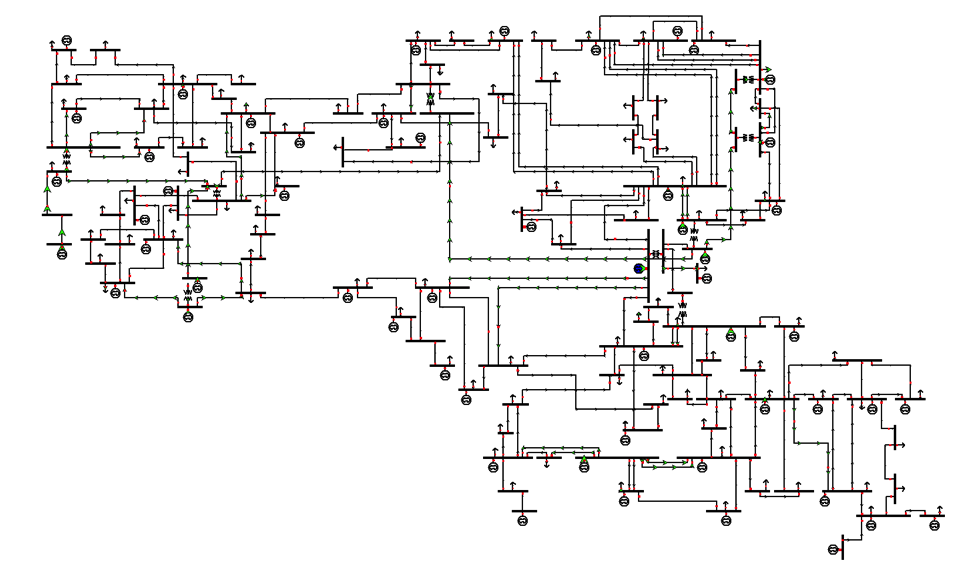
\includegraphics[width=\textheight]{IEEE118}
    \caption{IEEE 118 Power Grid}%
    \label{fig:ieee118}
  \end{figure}
\end{slide}

\begin{slide}{False Data Injection}
  \begin{columns}[c]
    \begin{column}{0.28\textwidth}
      \begin{itemize}
        \item 226 states
        \item 38 sensors
        \item Sparse dynamic matrix
      \end{itemize}
    \end{column}% \hfill%
    \begin{column}{0.68\textwidth}
      \begin{figure}[ht!] \centering
        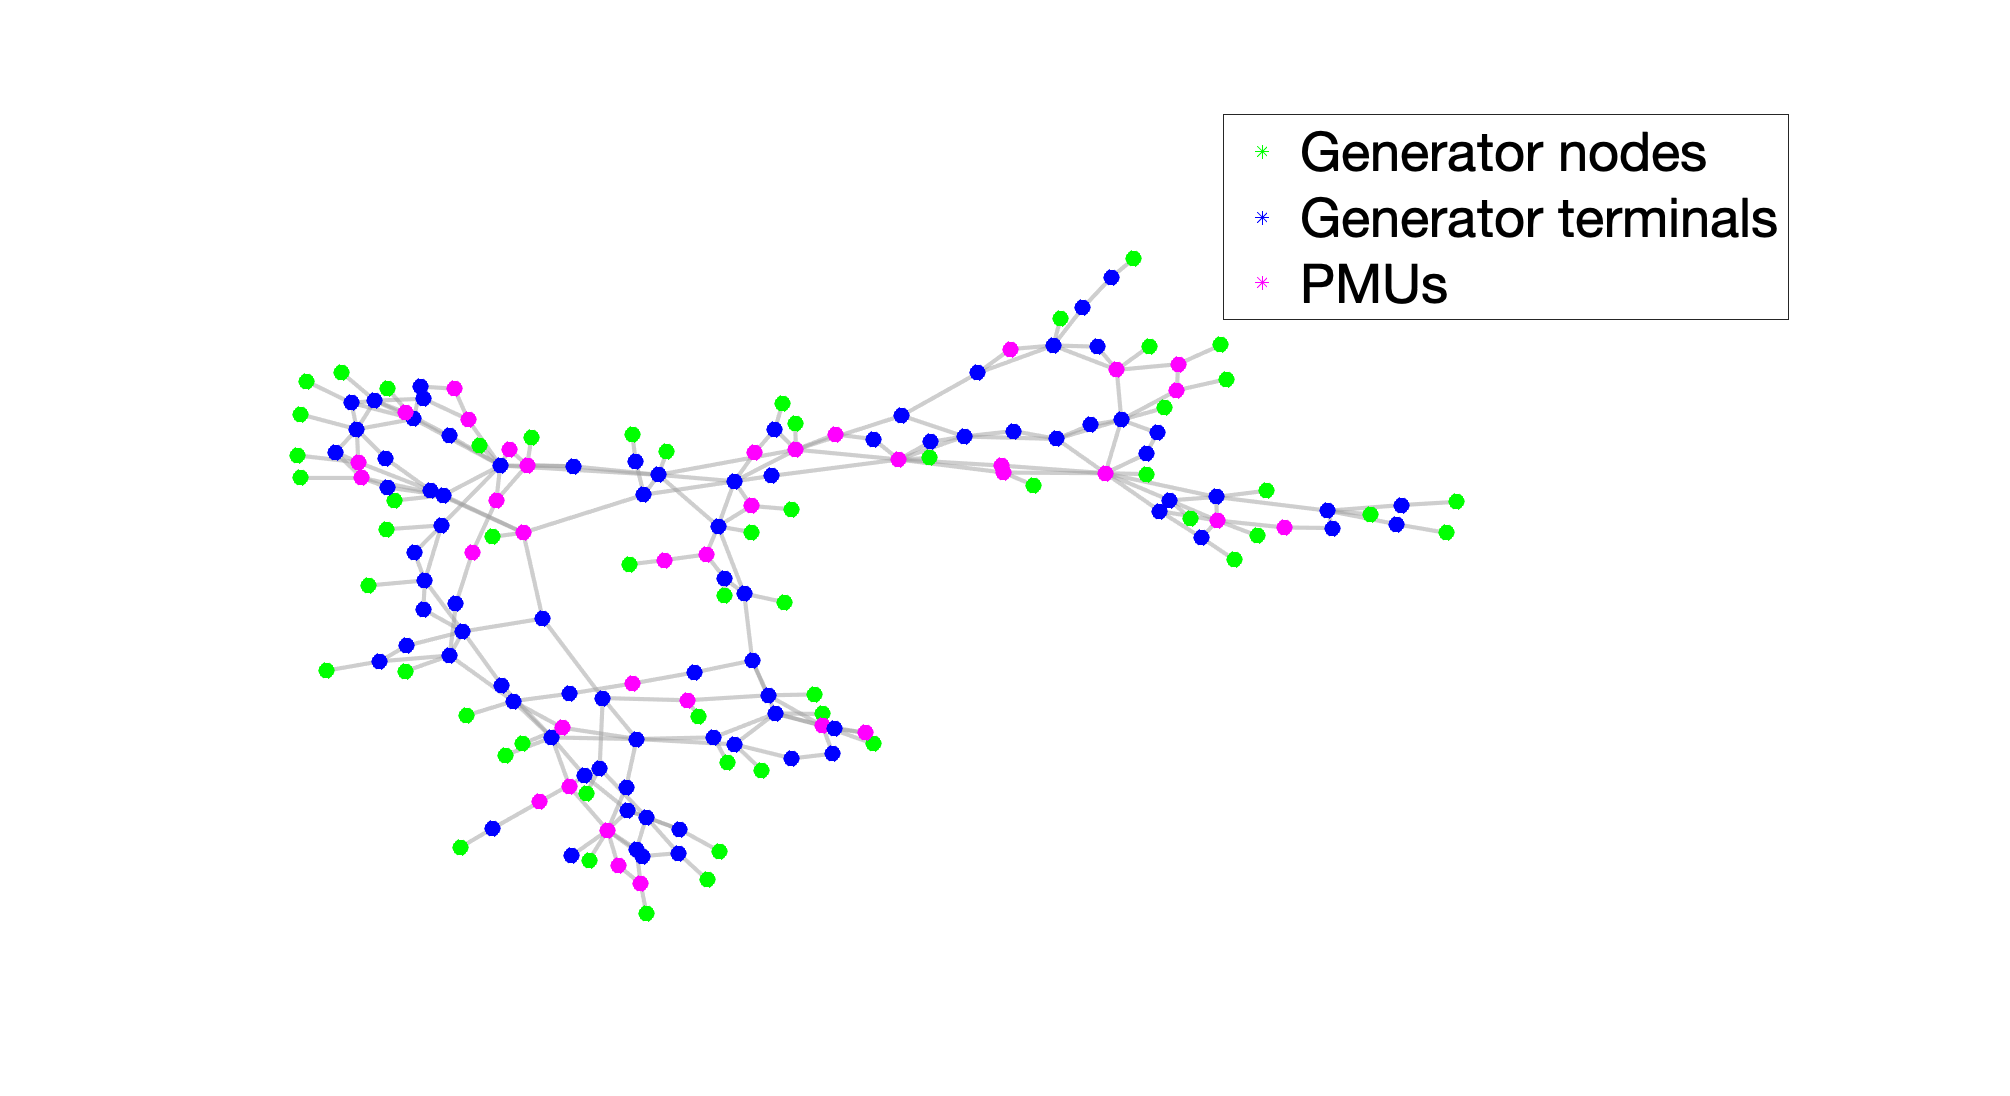
\includegraphics[width=\textheight]{graph-pg}
        \caption{IEEE 118 Power Grid's Dynamic Graph}%
        \label{fig:graph-pg}
      \end{figure}
    \end{column}%
  \end{columns}
\end{slide}

\begin{slide}{Functional Observer}
  \begin{columns}[c]
    \begin{column}{0.48\textwidth}
      \begin{itemize}
        \item \y{} are the measured outputs.
        \item \z{} are the states we wish to estimate.
        \item The observer has a reduced order dynamics system which is
              equivalent to the original one.
        \item Problem 1: how to find a \w{} that correctly estimates \z{}.
        \item Problem 2: how to find the observer's matrices \mN,\mJ,\mH and
              \mE.
      \end{itemize}
    \end{column}%
    \hfill%
    \begin{column}{0.48\textwidth}
      \begin{align}
        \begin{split}
          \dot{x}(t) & = Ax(t) + Bu(t) + Lf(t), \\
          \y         & = Cx(t),                 \\
          \z         & = Fx(t),
        \end{split} \\\nonumber\\
        \begin{split}
          \dw & = \mN\w + \mJ\y + \mH u(t), \\
          \hz & = \w + \mE\y.
        \end{split}
      \end{align}
    \end{column}%
  \end{columns}
\end{slide}

\begin{slide}{Observability}
  \begin{columns}[c]
    \begin{column}{0.48\textwidth}
      \begin{itemize}
        \item All desired states \z{} must be observable from the outputs \y.
        \item The observability of \((A,C,F)\) cannot be greater than that of
              \((A,C)\).
        \item There must be a path from every output \y{} to every output \z{}
              in the dynamics graph.
      \end{itemize}
    \end{column}%
    \hfill%
    \begin{column}{0.48\textwidth}
      \begin{equation}
        rank
        \begin{bmatrix}
          C \\ CA \\ F \\ FA
        \end{bmatrix}
        = rank
        \begin{bmatrix}
          C \\ CA \\ F
        \end{bmatrix}.
      \end{equation}
    \end{column}%
  \end{columns}
\end{slide}

\begin{slide}{Path Finder Algorithm}
  \begin{columns}[c]
    \begin{column}{0.48\textwidth}
      \begin{figure}[ht!]
        \centering 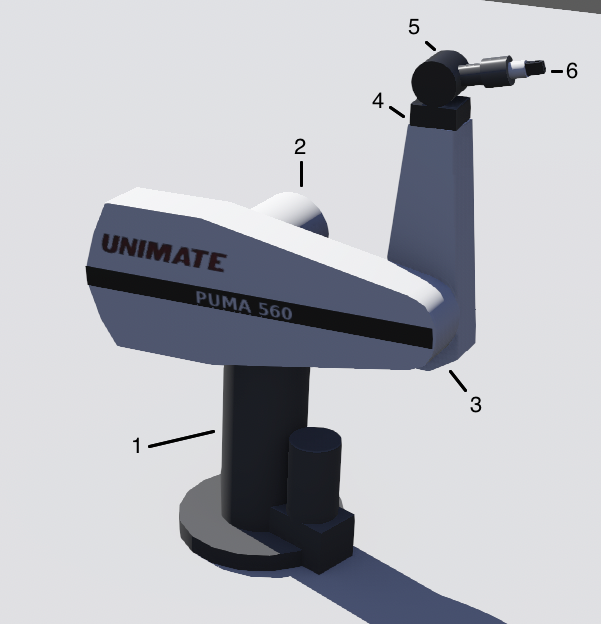
\includegraphics[width=0.8\textwidth]{puma560}
        \caption{Puma 560}%
        \label{fig:puma}
      \end{figure}
    \end{column}%
    \hfill%
    \begin{column}{0.48\textwidth}
      \begin{figure}[ht!]
        \centering
        \includegraphics[width=\textwidth]{graph-puma}
        \caption{Puma 560 dynamic's graph representation.}%
        \label{fig:puma-graph}
      \end{figure}
    \end{column}%
  \end{columns}
\end{slide}

% !TeX root = document.tex
% !TeX encoding = UTF-8 Unicode

\subsection{Observer Design}%
\label{subsec:observer-design}

\begin{slide}{Bank of Observers}
  \input{imgs/schematic}
\end{slide}

\begin{slide}{Observer Design}
  \begin{columns}[c]
    \begin{column}{0.55\textwidth}
      \begin{equation}
        \begin{aligned}
          \textrm{arg min } & \norm{P}_{2}    \\
          \textrm{s.t. }    & \dot{V} \prec 0 \\
                            & P \succ 0,
        \end{aligned}
      \end{equation}
      %
      where
      %
      \begin{align}
        \dot{V} \equiv & \begin{bmatrix}
                           X        & W  \\
                           W^{\top} & -I
                         \end{bmatrix},                                         \\
        \lambda\in     & \mathbb{R}^{+} \textrm{ is a free constant}, \nonumber \\
        P              & \textrm{ is a semidefinite positve matrix} \nonumber
      \end{align}
      %
      with
      %
      \begin{align}
        \begin{split}
          X = & \hat{A}^{\top}F^{\top}P - \hat{A}^{\top}C^{\top}\hat{E}^{\top} -                 \\
              & \hat{C}^{\top}\hat{K}^{\top} + PF\hat{A} - \hat{E}C\hat{A} - \hat{K}\hat{C} - \lambda{}I,
        \end{split} \\
        W = & \sqrt{\lambda}(PF - \hat{E}C).
      \end{align}
    \end{column}%
    \hfill%
    \begin{column}{0.55\textwidth}
      \begin{align}
        \begin{split}
          \hat{A} & = AF^{+},               \\
          \hat{C} & = CF^{+},               \\
          \hat{E} & = P\mE = PU + \hat{Y}V, \\
          \hat{K} & = PK,                   \\
          \hat{Y} & = PY.
        \end{split} \\\nonumber\\
        \begin{split}
          K   & = P^{-1}\hat{K},  \\
          Y   & = P^{-1}\hat{Y},  \\
          \mE & = U + YV,         \\
          R   & = F - \mE{}C,     \\
          \mN & = (RA - KC)F^{+}, \\
          \mJ & = K + N\mE{},     \\
          \mH & = RB.
        \end{split}
      \end{align}
    \end{column}%
  \end{columns}
\end{slide}

\begin{slide}{Observer Design Development}
  \begin{columns}[c]
    \begin{column}{0.55\textwidth}
      \begin{align}
        \begin{split}
          e & = \hat{z} - z   \\
            & = w + \mE{}y - Fx   \\
            & = w + \mE{}Cx - Fx.
        \end{split} \\
        \begin{split}
          \dot{e} & = \dot{w} + (\mE{}C-F)\dot{x}              \\
                  & = \mN{}w + \mJ{}y + \mH{}u + (\mE{}C-F)(Ax + Bu + Lf)  \\
                  & = \mN{}e + (\mN{}F-\mN{}\mE{}C+\mE{}CA-FA+\mJ{}C)x +           \\
                  & \phantom{=~} (\mH{}+\mE{}CB-FB)u + (\mE{}CL-FL)f.
        \end{split}
      \end{align}
    \end{column}%
    \hfill%
    \begin{column}{0.55\textwidth}
      \begin{align}
        \begin{split}
          \mN{} \textrm{ must be Hurwitz-stable}, &      \\
          \mN{}(F-\mE{}C)-(F-\mE{}C)A+\mJ{}C      & = 0, \\
          \mH{}-(F-\mE{}C)B                       & = 0.
        \end{split} \\\nonumber\\
        \begin{split}
          (F-\mE{}C)L_{i} & = 0,     \\
          (F-\mE{}C)L_{n} & \neq 0.
        \end{split}
      \end{align}
    \end{column}%
  \end{columns}
\end{slide}

\begin{slide}{Observer Design Development}
  \begin{columns}[c]
    \begin{column}{0.55\textwidth}
      \begin{align}
        V             & = e^{\top}Pe,              \\
        \dot{e}       & = \mN{}e-(F-\mE{}C)L_{n}f, \\
        e             & \propto L_{n}f,            \\
        \norm{L_{n}f} & = \lambda{}\norm{e},       \\
        R             & = F-\mE{}C,                \\
        \dot{e}       & = \mN{}e-R\lambda\norm{e}.
      \end{align}
    \end{column}%
    \hfill%
    \begin{column}{0.55\textwidth}
      \begin{align}
        \begin{split}
          \dot{V} & = \dot{e}^{\top}Pe + e^{\top}P\dot{e}                                             \\
                  & = (\mN{}e-\lambda{}R\norm{e})^{\top}Pe + e^{\top}P(\mN{}e-\lambda{}R\norm{e})     \\
                  & = e^{T}(\mN{}^{\top}P + P\mN{})e - 2\lambda\norm{e^{\top}PR}\cdot\norm{e}         \\
                  & \leq e^{T}(\mN{}^{\top}P + P\mN{})e - \lambda(\norm{e^{\top}PR}^{2}+\norm{e}^{2}) \\
                  & = e^{T}(\mN{}^{\top}P + P\mN{} - \lambda{}PRR^{\top}P - \lambda{}I)e.
        \end{split}
      \end{align}
    \end{column}%
  \end{columns}
\end{slide}

\begin{slide}{Observer Design Development}
  \begin{columns}[c]
    \begin{column}{0.55\textwidth}
      \begin{align}
        \begin{split}
          \mN{}(F-\mE{}C) & = RA-\mJ{}C,              \\
          \mN{}F          & = RA-(\mJ{}-\mN{}\mE{})C, \\
          K               & = \mJ{}-\mN{}\mE{},       \\
          \mN{}           & = RAF^{+}-KCF^{+},
        \end{split} \\
        \begin{split}
          (F-\mE{}C)L_{i} & = 0,                                              \\
          \mE{}CL_{i}     & = FL_{i},                                         \\
          \mE{}           & = FL_{i}(CL_{i})^{+} + Y(I-(CL_{i})(CL_{i})^{+}), \\
          U               & = \mE{}CL_{i}L_{i}^{+},                           \\
          V               & = I-L_{i}L_{i}^{+},                               \\
          \mE{}           & = U+YV.
        \end{split}
      \end{align}
    \end{column}%
    \hfill%
    \begin{column}{0.55\textwidth}
      \begin{align}
        \begin{split}
          \dot{V} & = e^{T}((R\hat{A} - \mE{}C\hat{A} - K\hat{C})^{\top}P +                                     \\
                  & P(R\hat{A} - \mE{}C\hat{A} - K\hat{C}) - \lambda{}PRR^{\top}P - \lambda{}I)e.               \\
                  & = \hat{A}^{\top}F^{\top}P - \hat{A}^{\top}C^{\top}\hat{E}^{\top} - \hat{C}^{\top}K^{\top} + \\
                  & PF\hat{A} - \hat{E}C\hat{A} - K\hat{C} - \lambda{}PRR^{\top}P - \lambda{}I.
        \end{split}
      \end{align}
    \end{column}%
  \end{columns}
\end{slide}

\begin{slide}{Residual Generator}
  \begin{columns}[c]
    \begin{column}{0.55\textwidth}
      \begin{align}
        r(t) & = Gw(t) + My(t), \\
        \begin{split}
          M & = (C(1-L_{i}))^{\top},      \\
          G & = -M(I-CF^{+}\mE{})^{-1}CF^{+},
        \end{split}
      \end{align}
    \end{column}%
    \hfill%
    \begin{column}{0.55\textwidth}
      \begin{align}
        \begin{split}
          r & = Gw + My                          \\
            & = Q(y - Cx)                        \\
            & = Q(y - CF^{-1}\hat{z})            \\
            & = Q(y - CF^{-1}(w+\mE{}y))         \\
            & = Q((I-CF^{-1}\mE{})y - CF^{-1}w),
        \end{split} \\
        \begin{split}
          M & = Q(I-CF^{-1}\mE{}), \\
          G & = -QCF^{-1}.
        \end{split}
      \end{align}
    \end{column}%
  \end{columns}
\end{slide}

% !TeX root = document.tex
% !TeX encoding = UTF-8 Unicode

\subsection{Results}%
\label{subsec:fo-results}

\begin{slide}{Results (Puma 560)}
  \begin{columns}[c]
    \begin{column}{0.55\textwidth}
      \begin{figure}[ht!]
        \centering
        \includegraphics[width=0.9\linewidth]{s7a2}
        \caption{Residuals for attack on sensor 7, with \(\delta=1\)}%
        \label{fig:s7a2}
      \end{figure}
    \end{column}%
    \hfill%
    \begin{column}{0.55\textwidth}
      \begin{figure}[ht!]
        \centering
        \includegraphics[width=0.9\linewidth]{s8a1}
        \caption{Residuals for attack on sensor 8, copying the values from
          sensor 9}%
        \label{fig:s8a1}
      \end{figure}
    \end{column}%
  \end{columns}
\end{slide}

\begin{slide}{Results (IEEE118)}
  Functional Observer with 120 states.
  \begin{columns}[c]
    \begin{column}{0.55\textwidth}
      \begin{figure}[ht!]
        \centering
        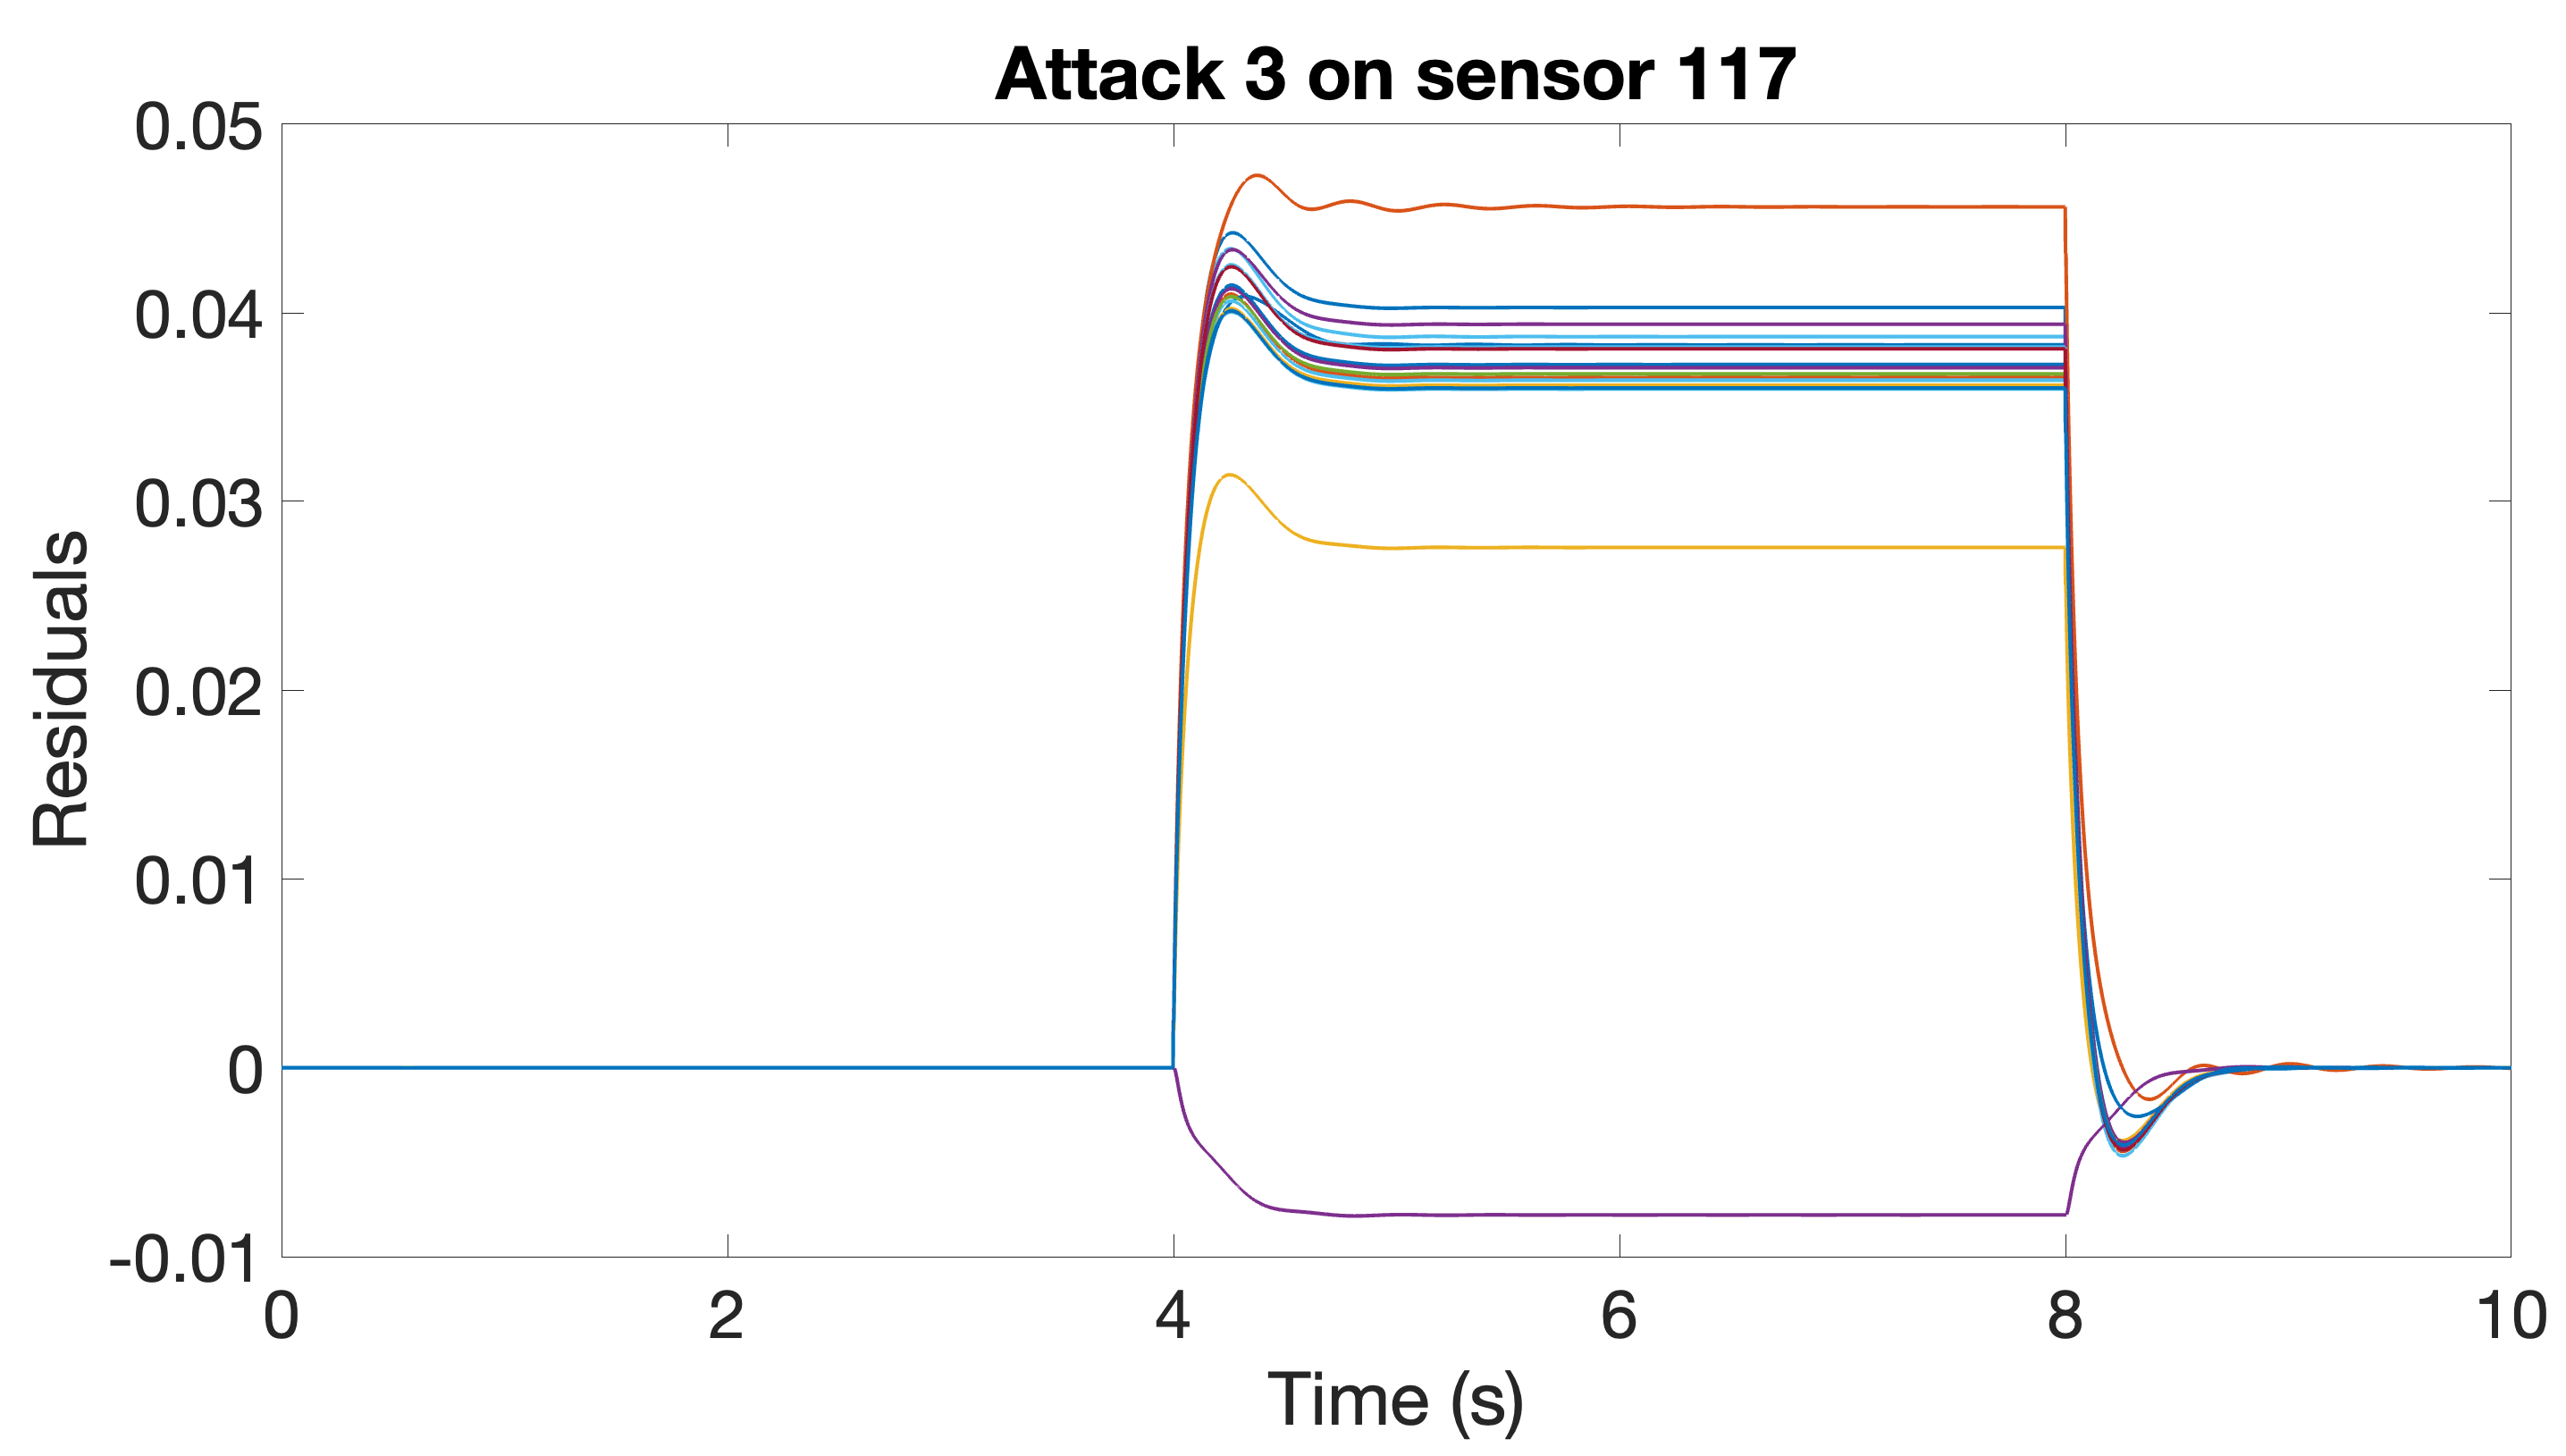
\includegraphics[width=0.9\linewidth]{s117a3}
        \caption{Residuals for multiplicative attack on state 117}%
        \label{fig:s117a3}
      \end{figure}
    \end{column}%
    \hfill%
    \begin{column}{0.55\textwidth}
      \begin{figure}[ht!]
        \centering
        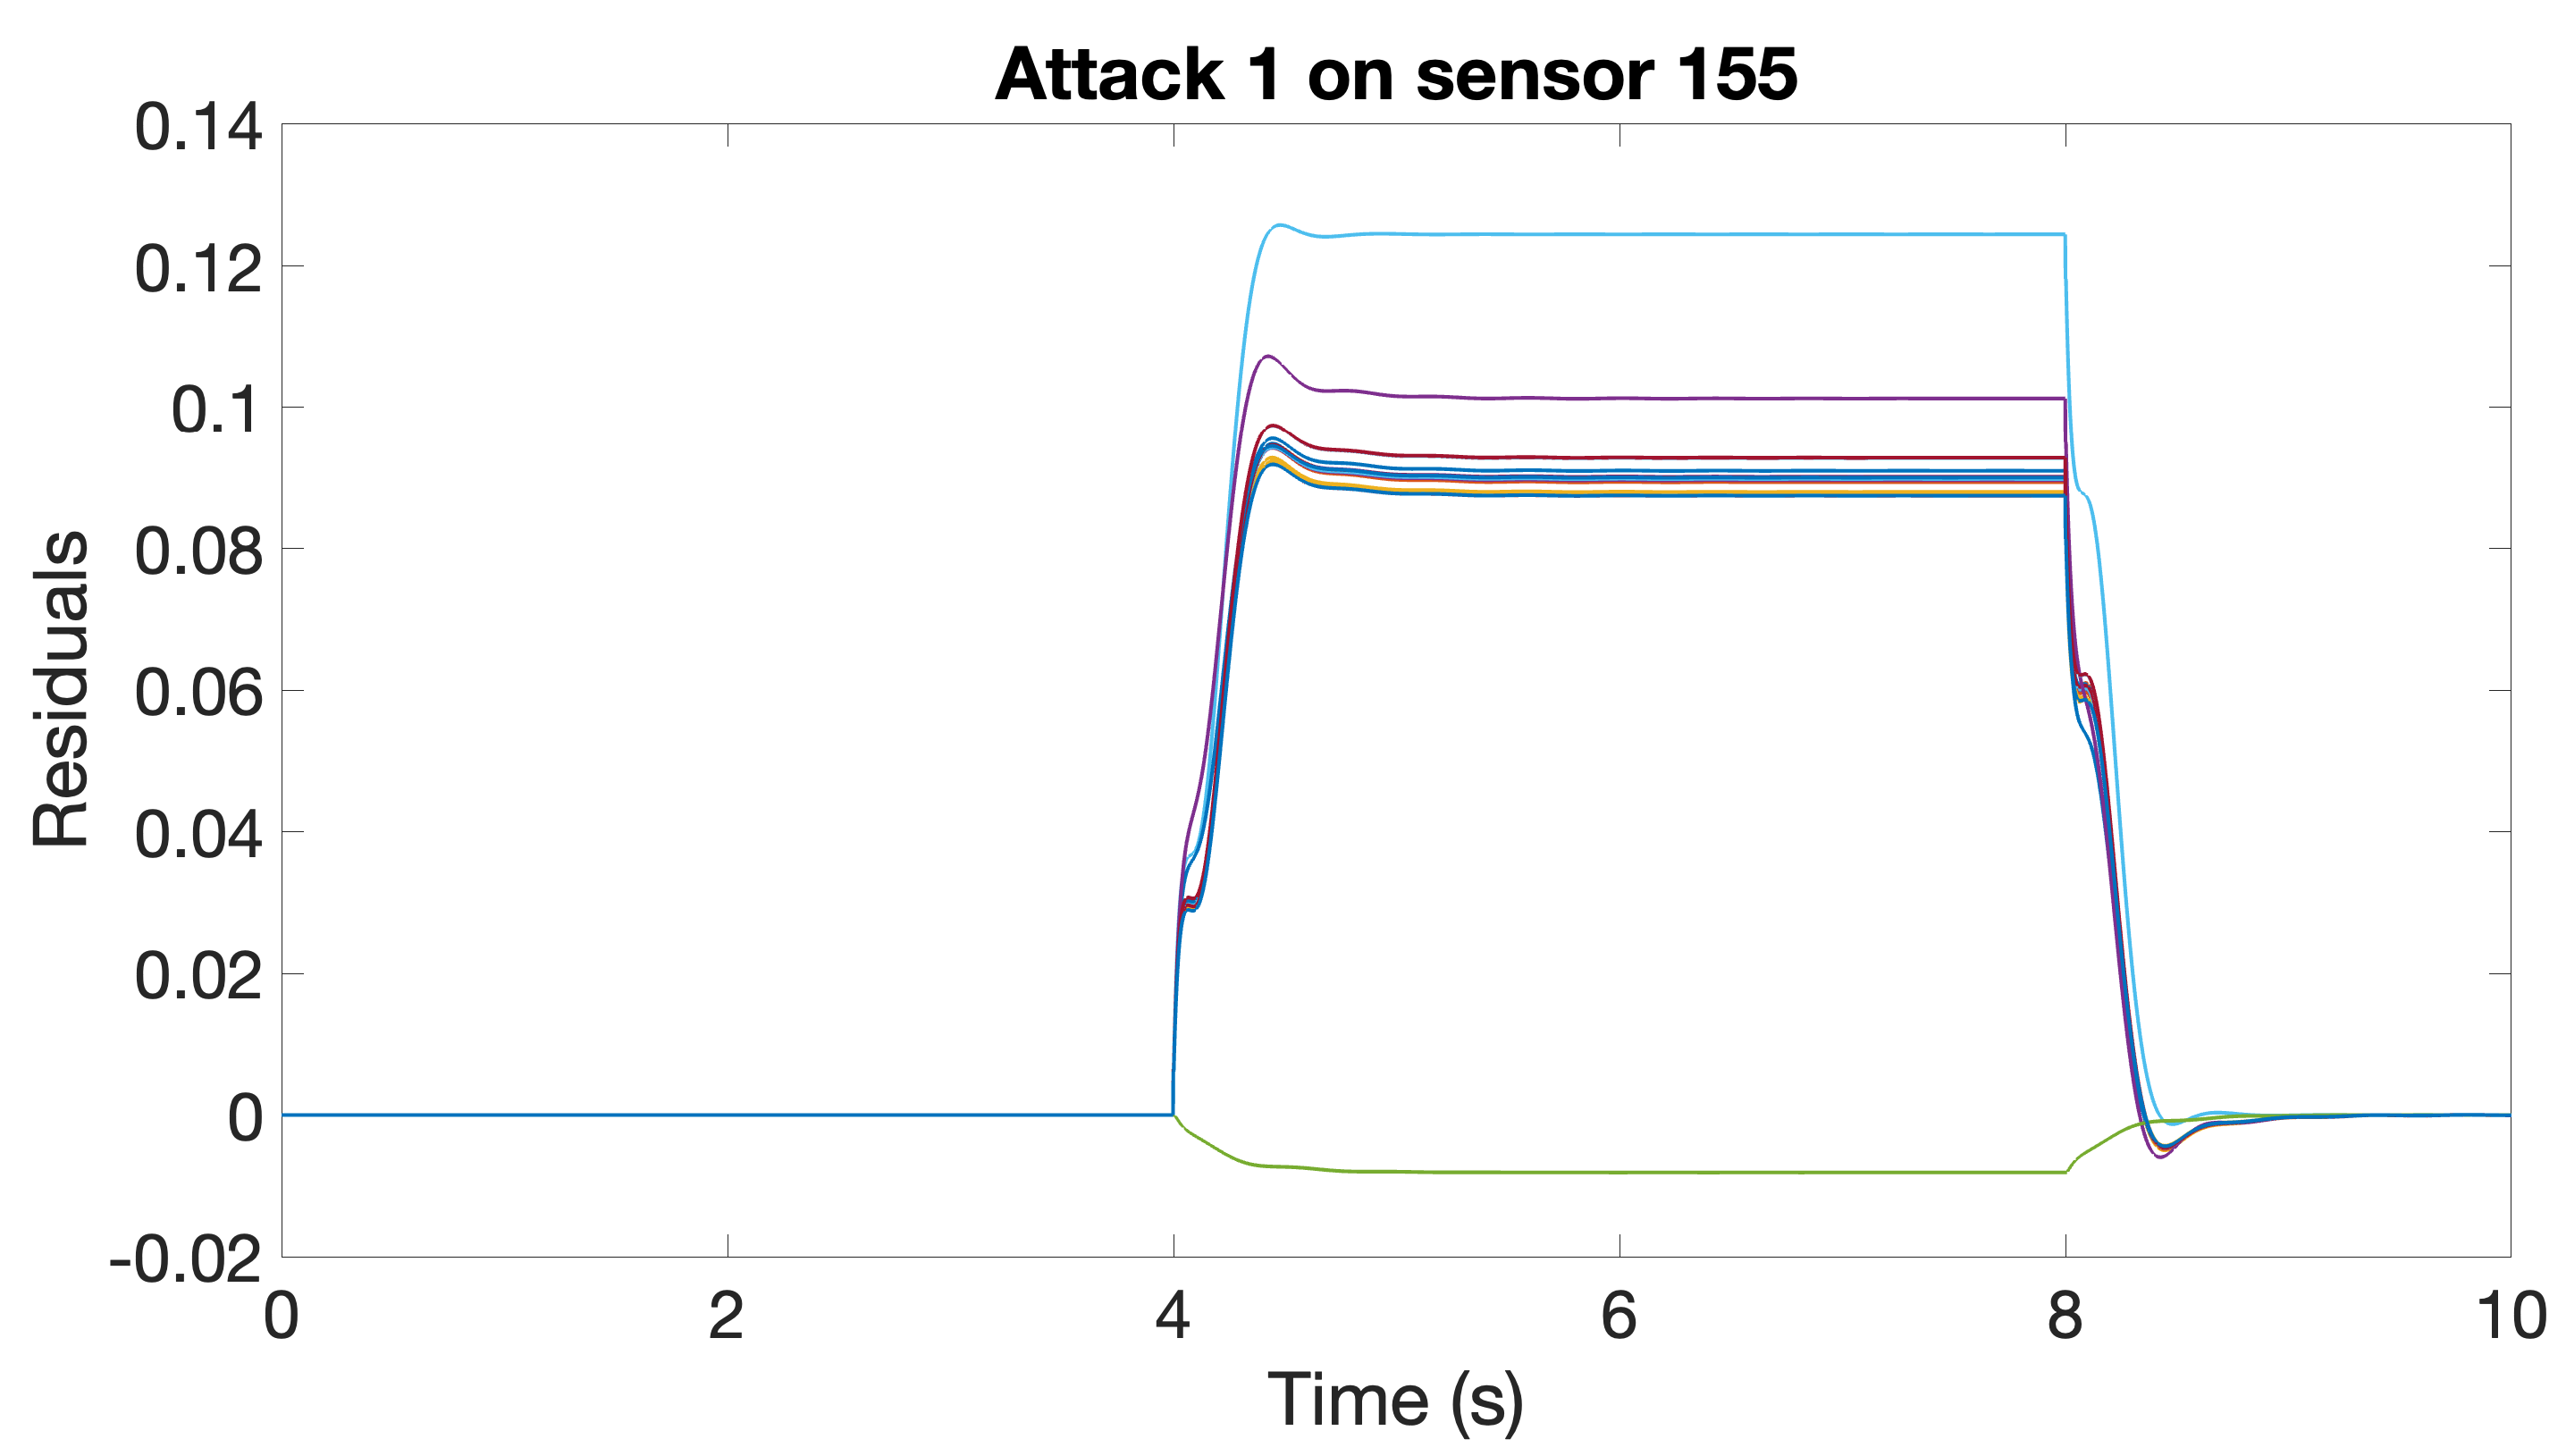
\includegraphics[width=0.9\linewidth]{s155a1}
        \caption{Residuals for state-copy attack on state 155}%
        \label{fig:s155a1}
      \end{figure}
    \end{column}%
  \end{columns}
\end{slide}

% !TeX root = document.tex
% !TeX encoding = UTF-8 Unicode

\subsection{Partial Conclusion}%
\label{subsec:fo-conclusion}

\begin{slide}{Partial Conclusion}
  \begin{itemize}
    \item The formulation is straightforward, optimization based and extendable.
    \item The example was a simple system for didactic reasons, but this kind of
          observer is better suited for large, sparse systems.
  \end{itemize}
\end{slide}


% !TeX root = document.tex
% !TeX encoding = UTF-8 Unicode

\section{Zero-Dynamics Attack}%
\label{sec:zda}

\subsection{Introduction}%
\label{subsec:ts-introduction}

\begin{slide}{}
  \usebeamercolor{frametitle}
  \vspace*{\fill}
  \begin{center}
    \textcolor{fg}{\Large{Zero-Dynamics Attack}}
  \end{center}
  \vspace*{\fill}
\end{slide}

\begin{slide}{Zero-Dynamics Attack}
  \begin{columns}[c]
    \begin{column}{0.48\textwidth}
      The attacker changes the control signal in a specific direction, taking
      advantage of the system's transmission zeros to change the system's states
      without affecting the system's output.
      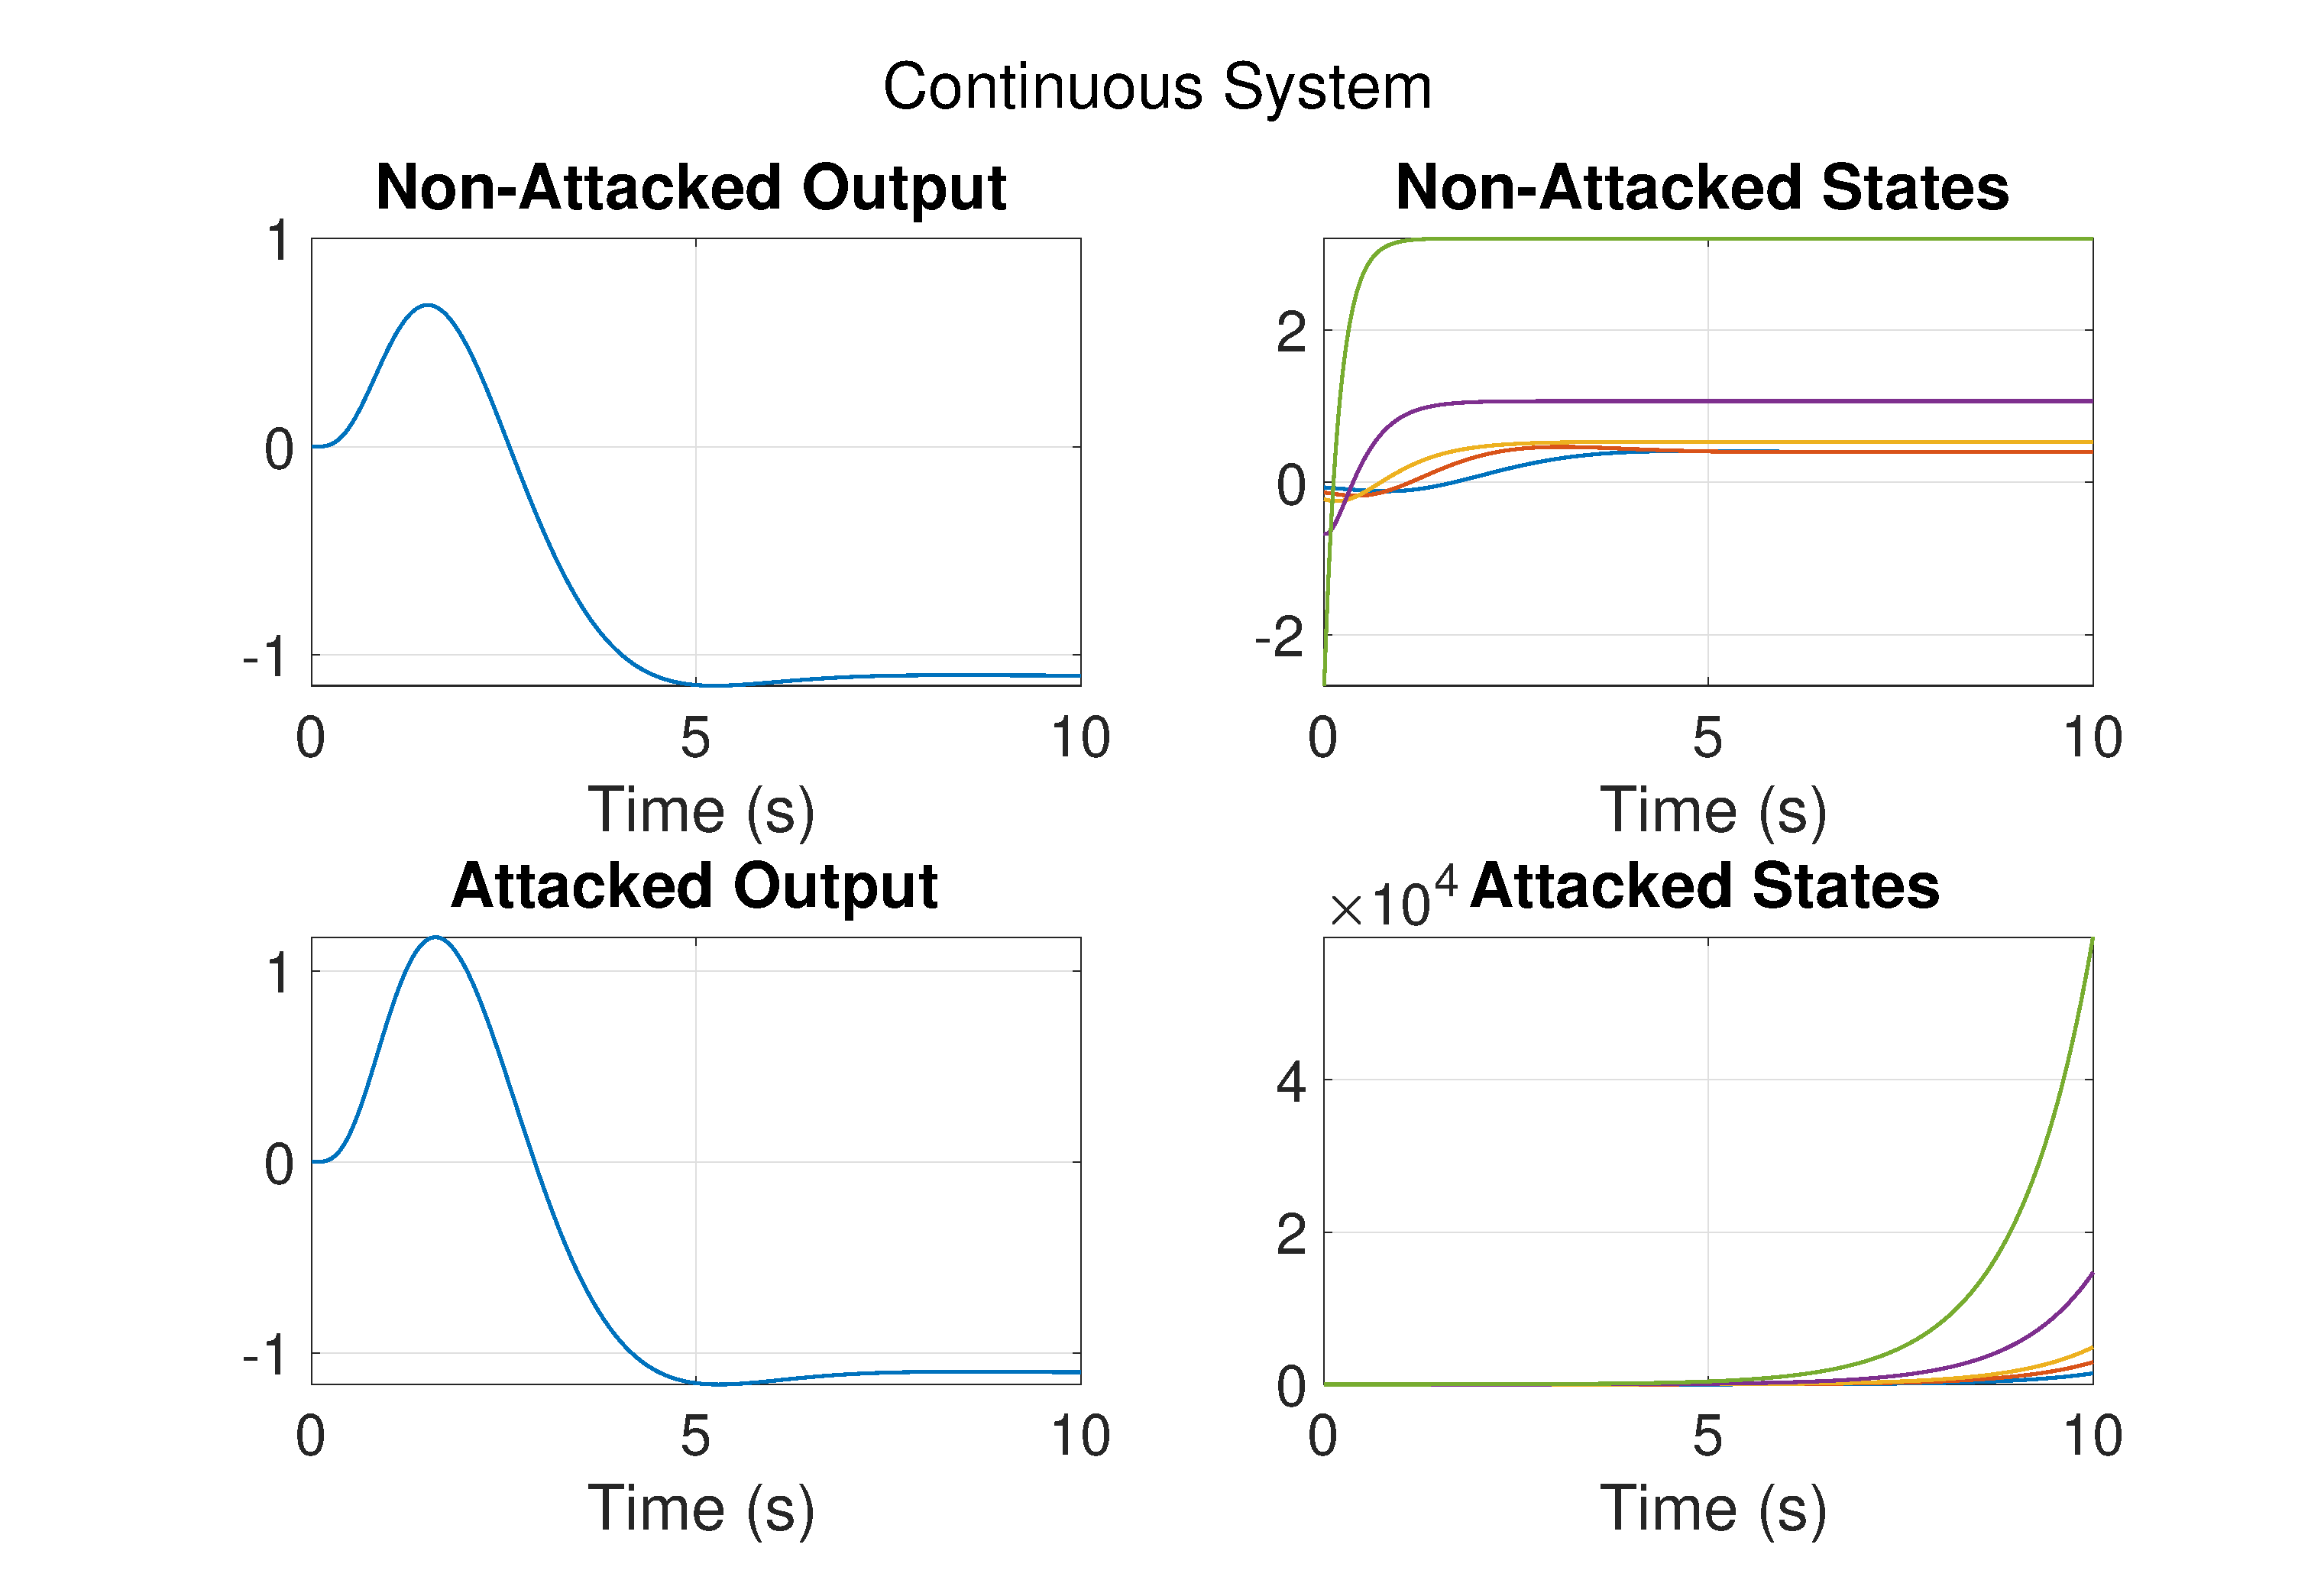
\includegraphics[width=\linewidth]{ct-system}
    \end{column}%
    \hfill%
    \begin{column}{0.48\textwidth}
      \begin{align}
        P(s)          & = \begin{bmatrix}
                            sI-A & -B \\
                            C    & D
                          \end{bmatrix},                                \\
        P(s_{0})z_{0} & = 0.                                            \\
        z_{0}         & = \begin{bmatrix} x_{0} \\ a_{0} \end{bmatrix}, \\
        a(t)          & = a_{0}e^{s_{0}t},                              \\
        \tilde{u}(t)  & =u(t) + a(t).
      \end{align}
    \end{column}%
  \end{columns}
\end{slide}

\begin{slide}{Zero-Dynamics Attack}
  Current detection schemes in the literature:\\~\\
  \begin{itemize}
    \item Generalized Zero-Order Holders
    \item Modified system models
    \item Schemes with multiple observers
  \end{itemize}
\end{slide}

\begin{slide}{Time-Scale Calculus}
  \begin{columns}[c]
    \begin{column}{0.48\textwidth}
      \begin{itemize}
        \item Unifies the continuous- and discrete-time calculi.
        \item Uses the so-called delta-derivative (\(\Delta\)-derivative).
        \item Exists for different time-sets, not only the continuous and
              discrete case.
      \end{itemize}
      \begin{figure}[ht!]
        \centering
        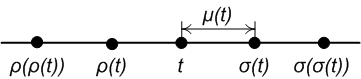
\includegraphics[width=0.6\linewidth]{ts-jump}
        \caption{Time-Scale jump operators. Source: \url{https://shorturl.at/bcJY1}}%
      \end{figure}
    \end{column}%
    \hfill%
    \begin{column}{0.48\textwidth}
      \begin{equation}
        \mathbb{T} = h\mathbb{Z} | \mathbb{R} | \mathbb{T}_{\textrm{iso}}
      \end{equation}
      %
      \begin{align}
        \textrm{forward:~}  & \sigma(t) = \inf\{\tau\in\mathbb{T}|\tau>t\}, \\
        \textrm{backward:~} & \rho(t) = \sup\{\tau\in\mathbb{T}|\tau<t\}.
      \end{align}
      %
      \begin{equation}
        \mu(t) = \sigma(t)-t \leftarrow \textrm{graininess}
      \end{equation}
      %
      \begin{equation}
        f(\sigma(t)) = f(t) + \mu(t)f^{\Delta}(t).
      \end{equation}
    \end{column}%
  \end{columns}
\end{slide}

\begin{slide}{Time-Scale System}
  \begin{columns}[c]
    \begin{column}{0.48\textwidth}
      \begin{itemize}
        \item Allows to evolve the system with arbitrary sampling-times.
        \item Has it own stability criteria based on the Hilger's circle.
      \end{itemize}
    \end{column}%
    \hfill%
    \begin{column}{0.48\textwidth}
      \begin{align}
        x^{\Delta}(t) & = A(\mu(t))x(t) + B(\mu(t))u(t),                      \\
        y(t)          & = Cx(t) + Du(t),                                      \\
        \phantom{1}   & \phantom{1}                                 \nonumber \\
        A(\mu(t))     & = \frac{e^{A\mu(t)}-I}{\mu(t)},                       \\
        B(\mu(t))     & = \int_{0}^{\mu(t)}\frac{e^{(\mu(t)-s)A}}{\mu(t)}Bds.
      \end{align}
    \end{column}%
  \end{columns}
\end{slide}

\begin{slide}{Stability Criteria}
  \begin{columns}[c]
    \begin{column}{0.48\textwidth}
      The system is stable if all of it's poles are within the Hilger's circle,
      defined as a the circle centered at \((-\frac{1}{\mu}, 0)\) and with
      radius \(\frac{1}{\mu}\).

      Note that the circle changes with the sampling-time (\(\mu\)).
    \end{column}%
    \hfill%
    \begin{column}{0.48\textwidth}
      \begin{figure}[ht!]
        \centering
        \resizebox{\linewidth}{!}{%
          \begin{tikzpicture}
            \fill [blue!40!white]           (0, 0) rectangle (1, 2);
            \draw [step=1cm,gray,very thin] (0, 0) grid      (2, 2);
            \node at (1, -0.25) {\(\dot{x}=f(x)\)};

            \fill [blue!40!white]           (3.5, 1) circle (0.5);
            \draw [step=1cm,gray,very thin] (3, 0)   grid   (5, 2);
            \node at (4, -0.25) {\(\Delta{}x=f(x)\)};

            \fill [orange!40!white]         (6.5, 1) circle (0.5);
            \fill [blue!40!white]           (6.6, 1) circle (0.4);
            \fill [green!40!white]          (6.7, 1) circle (0.3);
            \draw [step=1cm,gray,very thin] (6, 0)   grid   (8, 2);
            \node at (7, -0.25) {\(x^{\Delta{}}=f(x)\)};
          \end{tikzpicture}%
        }
        \caption{Different stability regions}%
        \label{fig:stability-regions}
      \end{figure}
    \end{column}%
  \end{columns}
\end{slide}

% !TeX root = document.tex
% !TeX encoding = UTF-8 Unicode

\subsection{Observer Design}%
\label{subsec:ts-observer-design}

\begin{slide}{Observer Design}
  \begin{columns}[c]
    \begin{column}{0.55\textwidth}
      \begin{itemize}
        \item Develop a Lyapunov-based LPV observer.
      \end{itemize}
    \end{column}%
    \hfill%
    \begin{column}{0.55\textwidth}
      \begin{figure}[ht!]
        \centering
        \resizebox{0.6\linewidth}{!}{%
          \begin{tikzpicture}[node distance=1cm,block/.style={align=center,draw,shape=rectangle,very thick,minimum height=2em, minimum width=3em},>=stealth]
            \node (C) [block]                             {Controller};
            \node (G) [block,above=1.5cm of C]            {System};
            \node (H) [block,above=of G]                  {Time-Scale Observer};
            \node (J) [block,above=of H]                  {Residual Generator};
            \node (u) [above left=0.5cm and 1cm of C]     {\(u(t)\)};
            \node (y) [above right=0.5cm and 1cm of C]    {\(y(t)\)};
            \node (r) [right=0.5cm of J]                  {\(r(t)\)};
            \node     [draw,rectangle,dashed,fit=(u) (y)] {Network};

            \draw [->,thick] (C) -| (u) |- (G);
            \draw [->,thick] (G) -| (y) |- (C);
            \draw [->,thick] (u) |- (H);
            \draw [->,thick] (y) |- (H);
            \draw [->,thick] (H) -- (J) -- (r);
          \end{tikzpicture}%
        }
        \caption{Observer's block diagram}%
        \label{fig:ts-schematic}
      \end{figure}
    \end{column}%
  \end{columns}
\end{slide}

\begin{slide}{Observer Design Development}
  \begin{columns}[c]
    \begin{column}{0.55\textwidth}
      \begin{align}
        x^{\Delta} & = Ax + Bu, \\
        y          & = Cx,
      \end{align}
      %
      \begin{gather}
        V = x\tr{}Px
      \end{gather}
      %
      \begin{gather}
        x(\sigma(t)) = x(t) + \mu(t)x^{\Delta}(t).
      \end{gather}
      %
      \begin{gather}
        PA + A\tr{}P + \mu{}A\tr{}PA \prec{} 0 \\
        P \succ{} 0
      \end{gather}
    \end{column}%
    \hfill%
    \begin{column}{0.55\textwidth}
      \begin{gather}
        \begin{bmatrix}
          M     & (PA - ZC)  \\
          \star & -\mu^{-1}P
        \end{bmatrix} \prec{} 0,  \\
        M = PA + A\tr{}P - ZC - C\tr{}Z\tr{}.
      \end{gather}
      %
      \begin{equation}
        Z = PL.
      \end{equation}
      %
      \begin{equation}
        x^{\Delta} = Ax + Bu -L(y - Cx).
      \end{equation}
    \end{column}%
  \end{columns}
\end{slide}

\begin{slide}{Observer Design Development}
  \begin{columns}[c]
    \begin{column}{0.55\textwidth}
      An LPV observer for a time-scale system of the form
      %
      \begin{align}
        \hat{x}^{\Delta} & = A(\mu)\hat{x} + B(\mu)u - L(\mu)(y - C\hat{x}),                                                                                                            \\
        L(\mu)           & = \sum_{i=0}^{3}\alpha_{i}(\mu)L_{i},                                                                                                                        \\
        \alpha_{0}(\mu)  & = \textcolor{frenchblue}{\frac{\bar{\mu}^{-1}-\mu^{-1}}{\bar{\mu}^{-1}-\ubar{\mu}^{-1}}}  \textcolor{flame}{\frac{\bar{\mu}-\mu}{\bar{\mu}-\ubar{\mu}}},  \\
        \alpha_{1}(\mu)  & = \textcolor{frenchblue}{\frac{\mu^{-1}-\ubar{\mu}^{-1}}{\bar{\mu}^{-1}-\ubar{\mu}^{-1}}} \textcolor{flame}{\frac{\bar{\mu}-\mu}{\bar{\mu}-\ubar{\mu}}},  \\
        \alpha_{2}(\mu)  & = \textcolor{frenchblue}{\frac{\bar{\mu}^{-1}-\mu^{-1}}{\bar{\mu}^{-1}-\ubar{\mu}^{-1}}}  \textcolor{flame}{\frac{\mu-\ubar{\mu}}{\bar{\mu}-\ubar{\mu}}}, \\
        \alpha_{3}(\mu)  & = \textcolor{frenchblue}{\frac{\mu^{-1}-\ubar{\mu}^{-1}}{\bar{\mu}^{-1}-\ubar{\mu}^{-1}}} \textcolor{flame}{\frac{\mu-\ubar{\mu}}{\bar{\mu}-\ubar{\mu}}},
      \end{align}
    \end{column}%
    \hfill%
    \begin{column}{0.55\textwidth}
      \begin{align}
                 & \begin{bmatrix}
                     M(\cubar{\mu},0) & PA(\cubar{\mu}) - Z_{0}C \\
                     \star            & -\frac{1}{\cubar{\mu}}P
                   \end{bmatrix} \prec{} 0,  \\
                 & \begin{bmatrix}
                     M(\cbar{\mu},1) & PA(\cbar{\mu}) - Z_{1}C \\
                     \star           & -\frac{1}{\cubar{\mu}}P
                   \end{bmatrix} \prec{} 0,    \\
                 & \begin{bmatrix}
                     M(\cubar{\mu},2) & PA(\cubar{\mu}) - Z_{2}C \\
                     \star            & -\frac{1}{\cbar{\mu}}P
                   \end{bmatrix} \prec{} 0, \\
                 & \begin{bmatrix}
                     M(\cbar{\mu},3) & PA(\cbar{\mu}) - Z_{3}C \\
                     \star           & -\frac{1}{\cbar{\mu}}P
                   \end{bmatrix} \prec{} 0,   \\
        M(\mu,i) & = PA(\mu) + A(\mu)\tr{}P - Z_{i}C - C\tr{}Z_{i}\tr,     \\
        L_{i}    & = P^{-1}Z_{i}.
      \end{align}
    \end{column}%
  \end{columns}
\end{slide}

% !TeX root = document.tex
% !TeX encoding = UTF-8 Unicode

\subsection{Results}%
\label{subsec:ts-results}

\begin{slide}{Results}
  \begin{columns}[c]
    \begin{column}{0.55\textwidth}
      \begin{figure}[ht!]
        \centering
        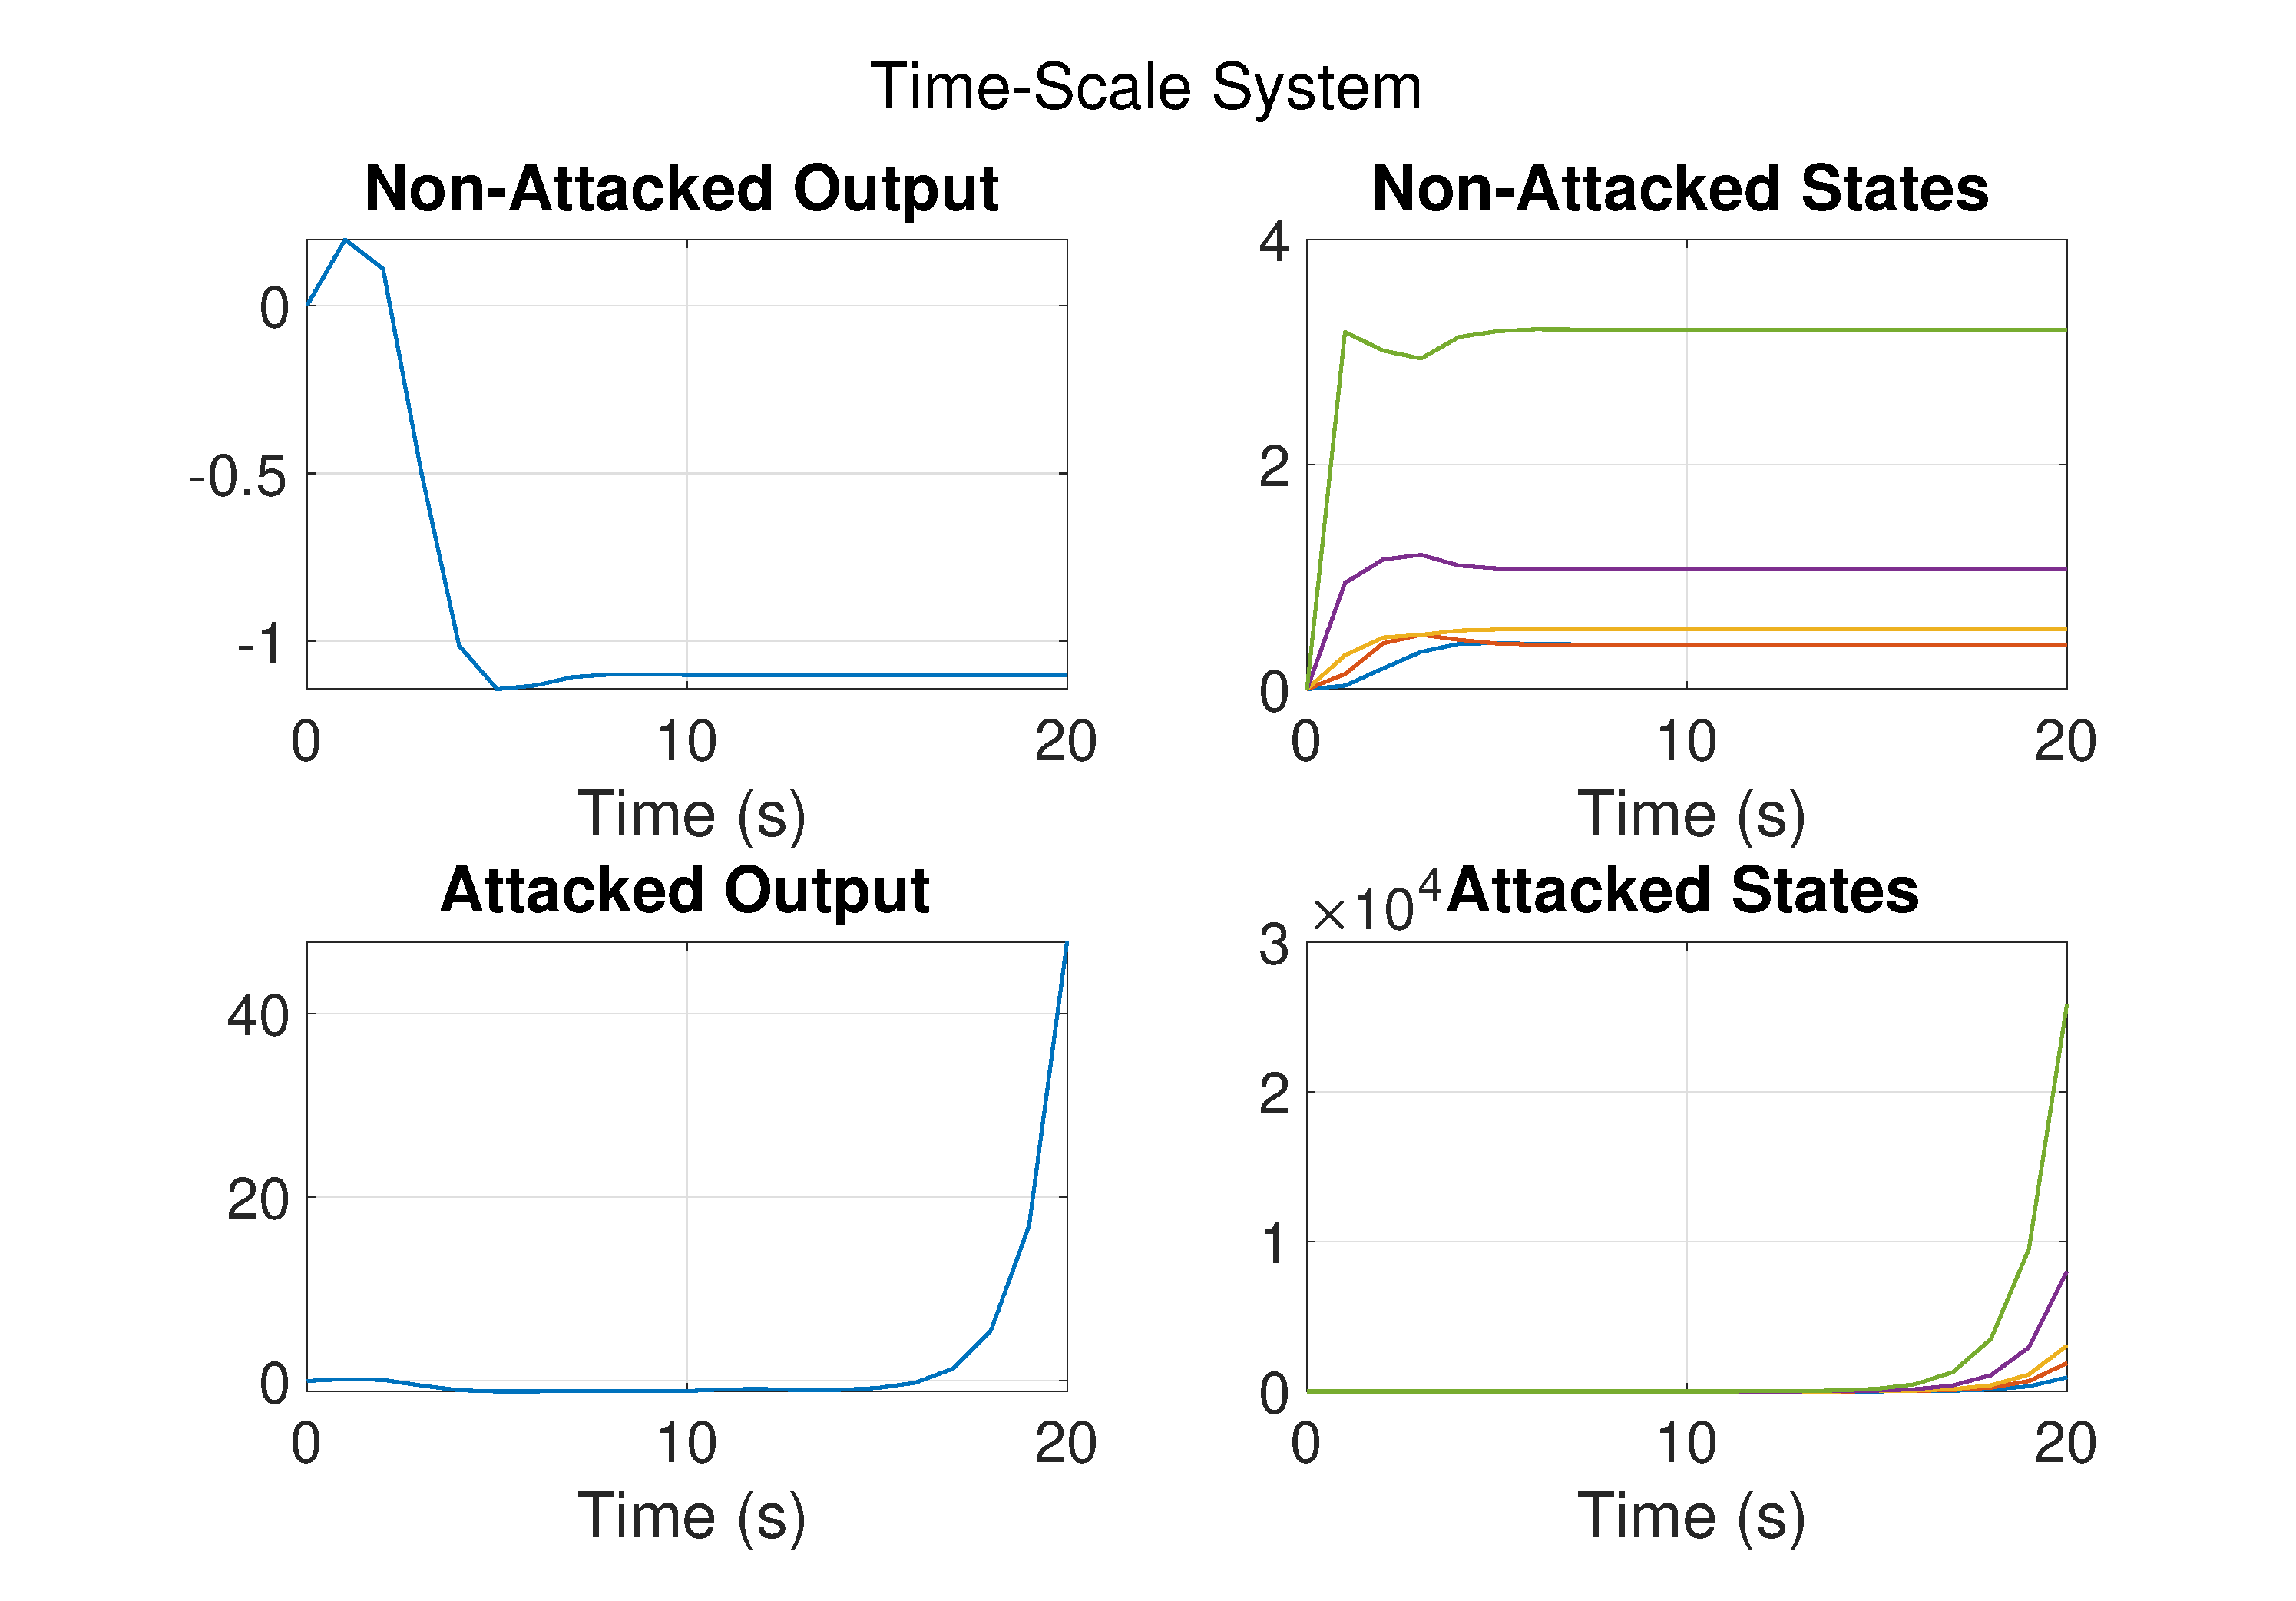
\includegraphics[width=\linewidth]{ts-system}
        \caption{Time-scale system's observer with \(\mu=\SI{1}{\second}\).}%
        \label{fig:ct-system}
      \end{figure}
    \end{column}%
    \hfill%
    \begin{column}{0.55\textwidth}
      \begin{figure}[ht!]
        \centering
        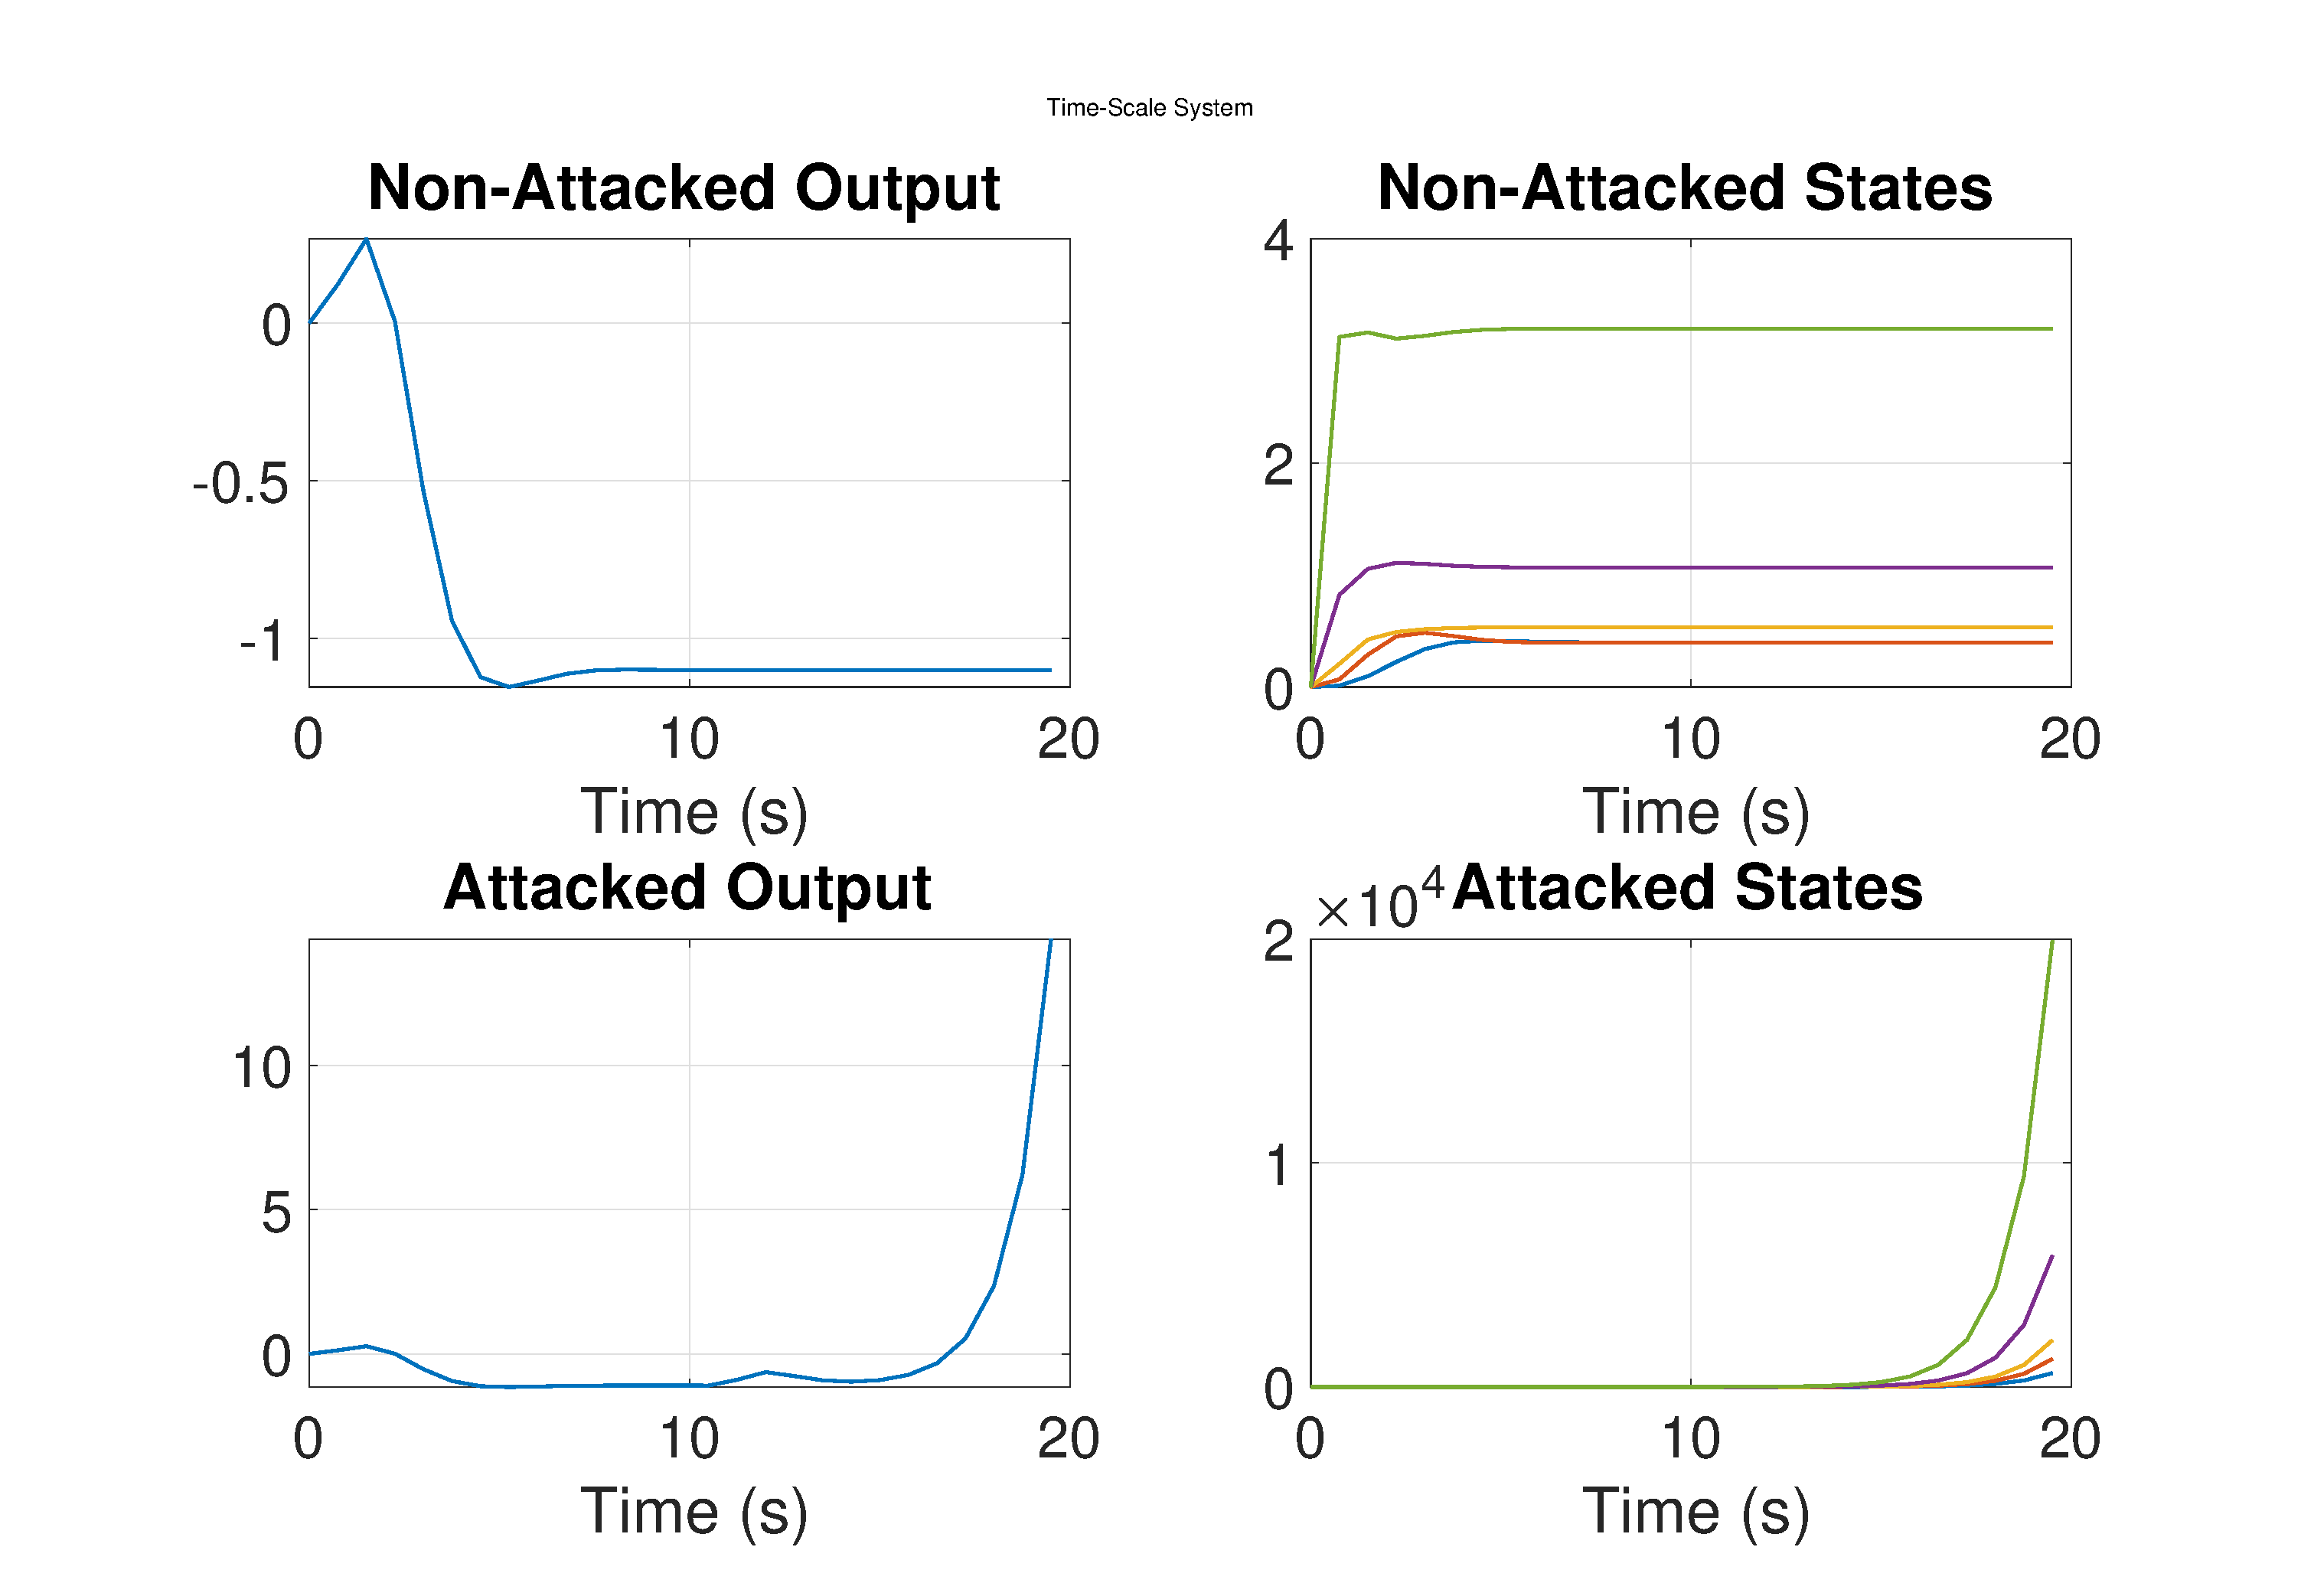
\includegraphics[width=\linewidth]{ts-system2}
        \caption{Time-scale system's observer with \(\mu=\SI{0.75}{\second}\).}%
        \label{fig:ts-system}
      \end{figure}
    \end{column}%
  \end{columns}
\end{slide}

% !TeX root = document.tex
% !TeX encoding = UTF-8 Unicode

\subsection{Partial Conclusion}%
\label{subsec:ts-conclusion}

\begin{slide}{Partial Conclusion}
  \begin{itemize}
    \item The formulation is straightforward, optimization based and extendable.
    \item The graininess \(\mu\) can change randomly to avoid attack vectors
          which may also affect the time-scale system. Better yet, techniques as
          the Game Theorie's Moving Target can give the best strategies to
          changing its value.
  \end{itemize}
\end{slide}


% !TeX root = document.tex
% !TeX encoding = UTF-8 Unicode

\section{Final Considerations}%
\label{sec:conclusion}

\begin{slide}{Future Works Perspective}
  \begin{itemize}
    \item Join the time-scale and functional-observer techniques.
    \item Make the resulting observer distributed.
  \end{itemize}
\end{slide}


\begin{slide}{}
  \usebeamercolor{frametitle}
  \vspace*{\fill}
  \begin{center}
    \textcolor{fg}{\Large{Merci pour votre attention.}}
  \end{center}
  \vspace*{\fill}
\end{slide}

\begin{slide}[allowframebreaks]{Referências}
  \nocite{*}
  \printbibliography{}
\end{slide}
\end{document}
